\documentclass[10pt, letterpaper]{article}
\usepackage{geometry}
\geometry{
 a4paper,
 total={170mm,257mm},
 left=20mm,
 top=20mm,
 }
\usepackage{graphicx} % Required for inserting images
\usepackage[english,greek]{babel}
\usepackage{mathabx} % Load the mathabx package
\usepackage{subcaption}
\usepackage{dirtytalk}
\usepackage{hyperref}
\usepackage{comment}
\usepackage{caption}
\usepackage{float}
\newcommand{\en}{\selectlanguage{english}}
\newcommand{\gr}{\selectlanguage{greek}}


\graphicspath{{../plots/}} % specify the path to the images

\title{Εργασία Θεωρίας Δικτύων }
\author{Φίλιππος Ρωσσίδης \\ (ΑΕΜ 10379)}
\date{\today}


\begin{document}
\maketitle


% !TeX spellcheck = gr


\section{Εισαγωγή}

Στην εργασία αυτή εξετάζουμε την αναγνώρηση κοινοτήτων. Συγκεκριμένα θα 
υλοποιούμε την 
\textlatin{distance quality function} και θα ελέγξουμε κατά πόσο αυτή είναι καλή
επιλογή. 

Οι συναρτήσεις αυτές (\textlatin{quality functions}) δέχονται ως όρισμα έναν
γράφο και μια κατανομή κοινοτήτων και επιστρέφουν μία τιμή. Σκοπός μας είναι 
να επιστρέφουν υψηλές τιμές για κατανομές που παρουσιάζουν ισχυρή κοινοτική συμπεριφορά,
ώστε να μπορούμε μεγιστοποιώντας αυτή τη συνάρτηση να ανιχνεύσουμε τις κοινότητες.

Θα υλοποιηθεί η συνάρτηση με έναν βέλτιστο ως προς τη ταχύτητα τρόπο, όπως και δύο αλγόριθμοι μεγιστοποίησής της. Θα υλοποιηθούν 
και κάποια \textlatin{benchmarks} ώστε να ποσοτικοποιηθεί η απόδοσή της και θα συγκριθεί με την εδραιωμένη μετρηκότητα \textlatin{modularity}.


\section{Η συνάρτηση \textlatin{distance quality}}

\subsection{Μαθηματικός Ορισμός}

Η συνάρτηση δέχεται σαν όρισμα έναν γράφο και κάποια κατανομή κοινοτήτων.

Ορίζουμε:

\[ D_V(i,j) = \min \{ k:A^k_G (i,j) \neq 0 \} \]
τον πίνακα που περιέχει τις αποστάσεις μεταξύ κάθε δύο κόμβων του γράφου 
$i,j$, όπου $A^k_G(i,j)$ ο πίνακας γειτνίασης του γράφου $G$. υψομένος στην $k$

δύναμη. 

Ορίζουμε επίσης:
\[ D_V(c) = \sum_{i,j \in c} D_V(i,j) \]

Αυτό αποτελεί μέτρο του πόσο στενά συνδεδεμένες είναι μεταξύ τους 
οι κοινότητες. Επιθυμούμε να το συγκρίνουμε με την αναμενώμενη τιμή 
για τυχαίο γράφο.

Για να ορίσουμε τον τυχαίο γράφο επιλέγουμε το γενικευμένο μοντέλο,
όπου συνδέουμε τυχαία ακμές μεταξύ κόμβων, διατηρώντας όμως τον βαθμό τους.


Αν $d_k(v)$ είναι ο $k$ βαθμός του κόμβου $v$, δηλαδή το πλήθος των 
ελάχιστων μονοματιών μήκους $k$ που ξεκινάν από τον $v$ και 
$m_k(G) = \frac{1}{2} \sum_{v \in V (G)} d_k(v)$ το πλήθος 
ελάχιστων μονοπατιών μήκους $k$ στον γράφο $G$, τότε η πιθανότητα δύο κόμβοι
$i,j \in G$ να συνδέονται με ακμή μήκους $k$ είναι:
\[ Pr[i,j,k] = \frac{d_k(i)}{2m_k(G)} \frac{d_k(j)}{2m_k(G)} \]
η αναμενώμενη απόσταση των κόμβων:
\[ \overline{D_V(i,j)} = \sum_{k=1}^{diam(G)} k Pr[i,j,k] \]
όπου $diam(G)$ η διάμετρος του γράφου (μέγιστο ελάχιστο μονοπάτι).

Αν ορίσουμε
\[ \overline{ D_V(c)  } = \frac{1}{2} \sum_{i,j \in c} \overline{ D_V(i,j) }\]
το άθροισμα των αναμενώμενων αποστάσεων των κόμβων στην κοινότητα $C$, 
τότε η συνάρτηση:

\[ Q_d(G,C) = \sum_{c \in C} (\overline{ D_V(c) } - D_V(c))\]
δηλώνει την επιθυμητή σύγκριση του μέτρου στενής σύνδεσης των κοινοτήτων 
$C$ ως προς του τυχαίου γράφου. 

Περιμένουμε οι τιμές της $Q_d$ να είναι υψηλές για ισχυρές δομές κοινοτήτων.


Στην υλοποίηση μου διάλεξα επίσης να τροποποιήσω την συνάρτηση ως εξίς:

\[ D_V(c) = \sum_{i,j \in c} D_V(i,j) \]
\[ \overline{ D_V(c)  } =  \sum_{i,j \in c} \overline{ D_V(i,j) }\]
\[ Q_d(G,C) = \sum_{c \in C} [(1 - \gamma)\overline{ D_V(c) } - \gamma D_V(c) ],  \ \ \ \ \gamma \in (0,1)\]

ώστε για $\gamma = 0.5$ να ισοδυναμεί με τον προηγούμενο ορισμό, αλλά να έχω 
δυνατότητα να επιλέξω ποιός όρος θα επηρεάσει περισσότερο.



\subsection{Υλοποίηση}  \label{ylop}


Χρησιμοποιήθηκε δυναμική προσέγγιση, δηλαδή οι τιμές του αλγορίθμου που χρησιμοποιούνται 
συχνά ($D_V(i,j), \ d_k(i), \ m_G(k), \ Pr[i,j,k],  \ \overline{D_V(i,j)},..$)
υπολογίζονται μία φορά στην αρχή και αποθηκεύονται ώστε να καλούνται σε σταθερό χρόνο στην πορεία. Έτσι γλυτώνουμε τις 
άσκοπες επαναλύψεις. 

Όπου είναι δυνατό χρησιμοποιούνται συναρτήσεις της βιβλιοθήκης $networkx$ μιας και 
είναι βελτιστοποιημένες και θα συμβάλουν στην ταχύτητα του κώδικα.

Στην πρώτη φάση του αλγορίθμου υπολογίζονται οι παρακάτω ποσότητες και αποθηκεύονται
για μελλοντική χρήση:
\begin{itemize}
    \item \textbf{διάμετρος του γράφου } 
    
    Χρησιμοποιείται η συνάρτηση της βιβλιοθήκης $networkx: diameter(G)$.
    
    \item  $\mathbf{D_V(i,j)}$
    
    Χρησιμοποιείται η συνάρτηση της βιβλιοθήκης $networkx: all\_pairs\_shortest\_path\_length(G)$,
    η οποία επιστρέφει απευθείας το ζητούμενο, την απόσταση κάθε δύο κόμβων του γράφου
    μεταξύ τους. Τα στοιχεία αποθηκεύονται σε ένα $python \ dict$.


    \item  $\mathbf{d_k(i)}$ \ και \ $\mathbf{m_G(k)}$
    
    Χρησιμοποιείται η συνάρτηση της βιβλιοθήκης $networkx:$ \\
    $ singe\_source\_shortest\_path\_length(G,source)$, η οποία υπολογίζει για κάποιον
    κόμβο $source$ όλα τα ελάχιστα μονοπάτια που τον έχουν σαν άκρο. Αν υπολογιστούν 
    αυτά τα μονοπάτια για κάθε κόμβο ως $source$ τότε θα έχουμε υπολογίσει
    όλα τα ελάχιστα μονοπάτια του γράφου δύο φορές (μία για $i \rightsquigarrow j$ και 
    μια για $j \rightsquigarrow i$).

    Τρέχουμε την παραπάνω συνάρτηση για κάθε κόμβο του γράφου ($source$). Στο $dict$ που 
    αυτή επιστρέφει, περιέχονται για κάθε άλλο κόμβο  ($target$) μια λίστα με μήκη από όλα
    τα μονοπάτια που τους ενώνουν ($source \rightsquigarrow target$). Έτσι για κάθε 
    μονοπάτι που βρίσκουμε στη λίστα, έχουμε το μήκος του $k$, 
    αυξάνουμε κατά $1$ τον βαθμό $d_k(source)$ και κατά $0.5$ τη τιμή 
    $m_G(k)$. Χρησιμοποιούμε $0.5$ διότι $m_k(G) = \frac{1}{2} \sum_{v \in V (G)} d_k(v)$
    (μετράμε κάθε μονοπάτι $2$ φορές).


    \item $\mathbf{Pr[i,j,k]}$  \ και \   $\mathbf{\overline{D_V(i,j)}}$
    
    Υπολογίζονται απλά με τους τύπους:
    \[ Pr[i,j,k] = \frac{d_k(i)}{2m_k(G)} \frac{d_k(j)}{2m_k(G)} \]
    \[ \overline{D_V(i,j)} = \sum_{k=1}^{diam(G)} k Pr[i,j,k] \]
    και αποθηκεύονται. 
    
    Συγκεκριμένα οι πίνακες αυτοί είναι συμμετρικοί (αφού 
    $\frac{d_k(i)}{2m_k(G)} \frac{d_k(j)}{2m_k(G)} = \frac{d_k(j)}{2m_k(G)} \frac{d_k(i)}{2m_k(G)}$)
    οπότε οι τιμές αυτές υπολογίζονται μία φορά για κάθε ζευγάρι $i,j$ και προστίθονται
    στο τέλος μία φορά για $i=j$ και δύο για $i \neq j$.
    


\end{itemize}

Προσοχή χρειάζεται το γεγονός ότι οι παραπάνω διαδικασίες δε μπορούν 
να λειτουργήσουν για μη συνδεδεμένους γράφους. Έτσι υιοθετούμε τη σύμβαση ότι 
δύο μη συνδεδεμές συνεκτικές συνιστώσες δεν μπορούν να βρίσκονται στην ίδια 
κοινότητα. Όποτε διαχωρίζουμε τον γράφο στις συνεκτικές του συνιστώσες και 
τρέχουμε τα παραπάνω για κάθε μία ξεχωριστά. Αυτή η προσέγγιση διατηρεί την 
πολυπλοκότητα ίδια (αφού οι συνεκτικές συνιστώσες διαμερίζουν τον γράφο).

\bigskip



\bigskip

Στη δεύτερη φάση του αλγορίθμου, αφού έχουν αποθηκευτεί τα παραπάνω, 
υπολογίζονται για τις δοσμένες κοινότητες $C$ τα αθροίσματα: 


\[ D_V(C) = \sum_{i,j \in C} D_V(i,j), \qquad \overline{ D_V(C)  } =  \sum_{i,j \in C} \overline{ D_V(i,j) }\]
 για $i,j \in C$, και η τιμή:
\[ Q_d(G,C) = \sum_{c \in C} [(1 - \gamma)\overline{ D_V(C) } - \gamma D_V(C) ]\]


\bigskip

\emph{Συνολική πολυπλοκότητα της δεύτερης φάσης: $O(|V|^2)$.}

\bigskip




\subsubsection{Μια πρώτη ματία στα αποτελέσματα}

\captionsetup[subfigure]{width=0.7\textwidth}


\begin{figure}[H]
  \begin{subfigure}{0.5\textwidth}
    \centering 
    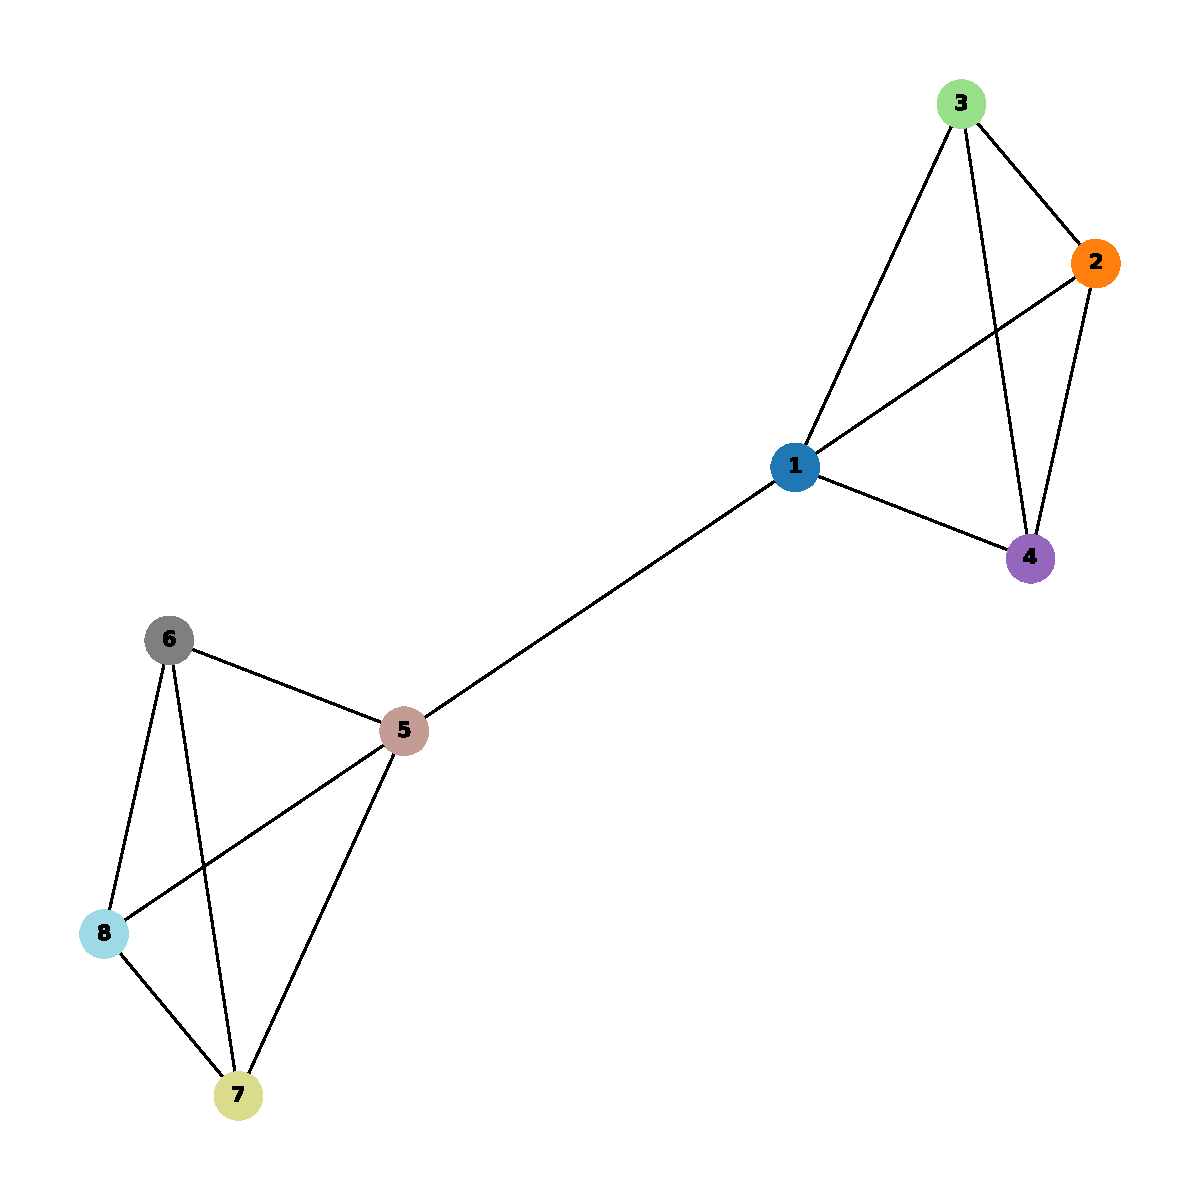
\includegraphics[width=0.68\linewidth]{quad_comm_gamma=0.5.pdf}
    \caption{Αποτελέσματα ωμής δύναμης για $\gamma = 0.5$. Κάθε κόμβος βρίσκεται σε δική του κοινότητα.}
    \label{fig:graph8comm}
  \end{subfigure}
  \begin{subfigure}{0.5\textwidth}
    \centering 
    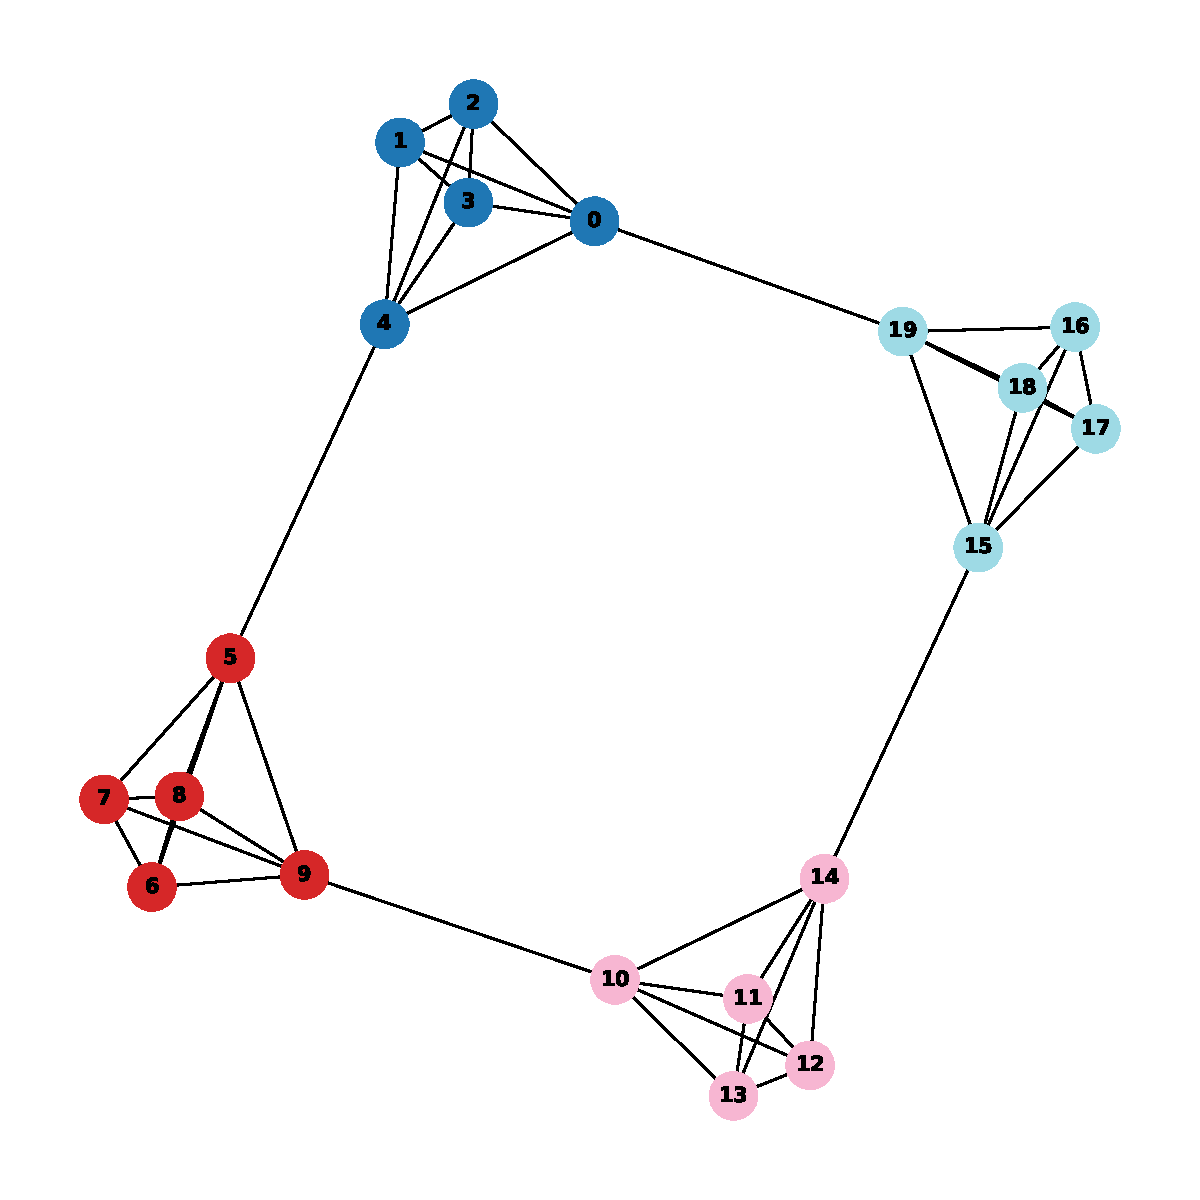
\includegraphics[width=0.75\linewidth]{cluster_4,5gamma=0.02,newman.pdf}
    \caption{Αποτελέσματα αλγορίθμου \textlatin{Newman} για $\gamma = 0.02$. Οι κοινότητες έχουν αναγνωριστεί σωστά.}
    \label{fig:newman4,5}
  \end{subfigure}
  \caption{}
  \label{}
\end{figure}





Για μια πρώτη εικόνα της λειτουργίας της παραπάνω μετρηκής, δοκιμάστηκε τεχνική ωμής δύναμης σε διάφορους γράφους,
για $\gamma = 0.5$ (δηλαδή τον αρχικό ορισμό της).
Ένα παράδειγμα βρίσκεται στο σχήμα \ref{fig:graph8comm}, όπου κάθε κοινότητα χρωματίζεται με δικό της χρώμα. 

Στο σχήμα φαίνονται οι κοινότητες για τις οποίες η τιμή $Q_d$ είναι μέγιστη. Ενώ περιμέναμε για τον γράφο αυτό να επιστραφούν 
δύο κοινότητες των 4 κόμβων, βλέπουμε ότι αυτό δεν συμβαίνει. Συγκεκριμένα για $\gamma = 0.5$ βρέθηκε πειραματικά ότι 
τη μέγιστη τιμή $Q_d$ παίρνουμε πάντα όταν κάθε κόμβος έχει δική του κοινότητα. Σε αυτό θα χρησιμεύσει η τιμή $\gamma$, όπου με την 
αλλαγή της μπορούμε να έχουμε την επιθυμητή συμπεριφορά (βλ. ενότητα \ref{gamma}).

Παρατίθεται προκαταβολικά στο σχήμα \ref{fig:newman4,5} το αποτέλεσμα του αλγορίθμου \textlatin{Newman} για $\gamma = 0.02$ για να φανεί 
το γεγονός αυτό.





\pagebreak




\section{Αλγόριθμοι μεγιστοποίησης του $Q_d$}



\subsection{Πρώτη προσπάθεια άπληστου αλγορίθμου}

Θα περιγράψω τον πρώτο αλγόριθμο που υλοποιήθηκε συνοπτικά, διότι παρότι αντικαταστάθηκε 
από αυτόν του \en Newman, \gr παρουσιάζει κάποια διαφορά στην λογική και τα αποτελέσματα:

\begin{enumerate}
  \item Υπολογίζουμε τις απαραίτητες ποσότητες και τις αποθηκεύουμε \\ ($D_V(i,j), \ d_k(i), \ m_G(k), \ Pr[i,j,k],  \ \overline{D_V(i,j)},diam(G)$).
  \item Αρχικοποιούμε κάθε κόμβο σε δική του κοινότητα.
  \item Για κάθε κόμβο, βρίσκουμε τον γειτονικό του κόμβο στου οποίου την κοινότητα 
  εάν μεταφερθεί θα υπάρχει η μέγιστη μεταβολή στο $Q_d$. Εάν η μεταβολή αυτή είναι θετική,
  τότε τον μεταφέρουμε σε εκείνη την κοινότητα.
  \item Επαναλαμβάνουμε το βήμα 3 μέχρι να μην γίνεται καμία μεταβολή.
\end{enumerate}

Ο αλγορίθμος αυτός δέχεται βελτιστοποίηση, ειδικότερα στο κομμάτι όπου 
υπολογίζει την ποσότητα $Q_d$ για κάθε μεταβολή τον κόμβων σε κοινότητες. 
Ένα μεγάλο μέρος της εξίσωσης $Q_d(G,C) = \sum_{c \in C} [(1 - \gamma)\overline{ D_V(c) } - \gamma D_V(c)]$
παραμένει σταθερό όταν μετακινούμε μόνο έναν κόμβο και κρατάμε τις υπόλοιπες κοινότητες
σταθερές, και το γεγονός αυτό θα εκμεταλευτούμε στη συνέχεια.

Επίσης εδώ τίθεται το ζήτημα της σύγκλισης, δηλαδή το πόσο γρήγορα ο αλγόριθμος συγκλίνει στην βέλτιστη λύση (εξαρτάται από 
τη τιμή του $\gamma$), το οποίο λύνεται στην συνέχεια.

% αποτελεσματα 

\subsubsection{Απόδοση}

Θα περιγραφτεί εδώ η διαδικασία με την οποία μετρήθηκε η απόδοση του αλγορίθμου, η 
οποία θα χρησιμοποιηθεί και στη συνέχεια για τον αλγόριθμο του \en Newman. \gr

Αρχικά δημιουργείται ένας γράφος ο οποίος αποτελέιται από 4 πλήρεις υπογράφους 
των 5 κόμβων
συνδεδεμένους με μία ακμή μεταξύ τους σε μορφή κύκλου (σχήμα \ref{fig:fullcluster}).
Σε αυτόν τον γράφο περιμένουμε οι κοινότητες να είναι οι τέσσερεις πλήρεις υπογράφοι.


\begin{figure}[H]
  \begin{subfigure}{0.5\textwidth}
    \centering
    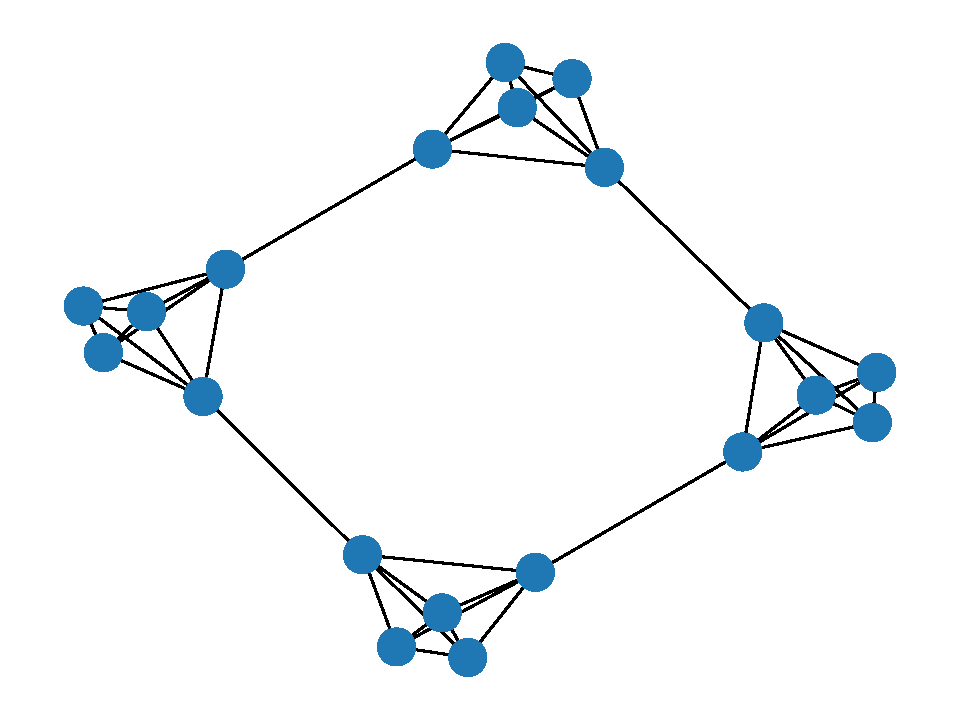
\includegraphics[width=0.6\linewidth]{fullcliustergraph.pdf}
    \caption{Αρχικός γράφος \en benchmark \gr}
    \label{fig:fullcluster}
  \end{subfigure}
  \begin{subfigure}{0.5\textwidth}
    \centering
    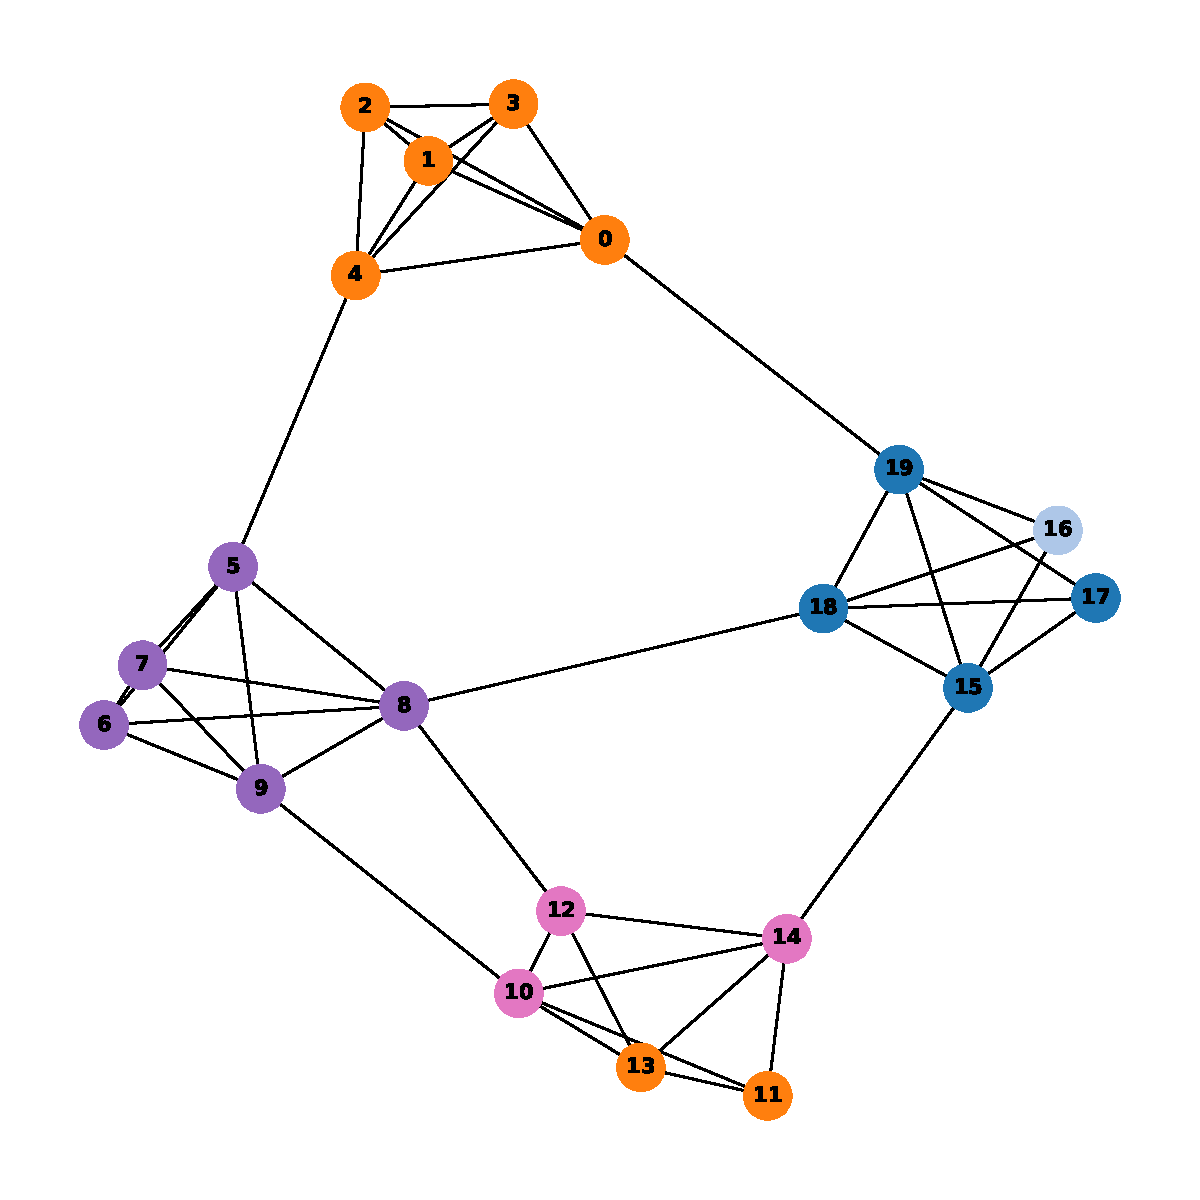
\includegraphics[width=0.6\linewidth]{iterations=1.pdf}
    \caption{2ο βήμα}
    \label{fig:it1}
  \end{subfigure}
  \caption{}
  \label{}
\end{figure}

\begin{figure}[H]
  \begin{subfigure}{0.5\textwidth}
    \centering
    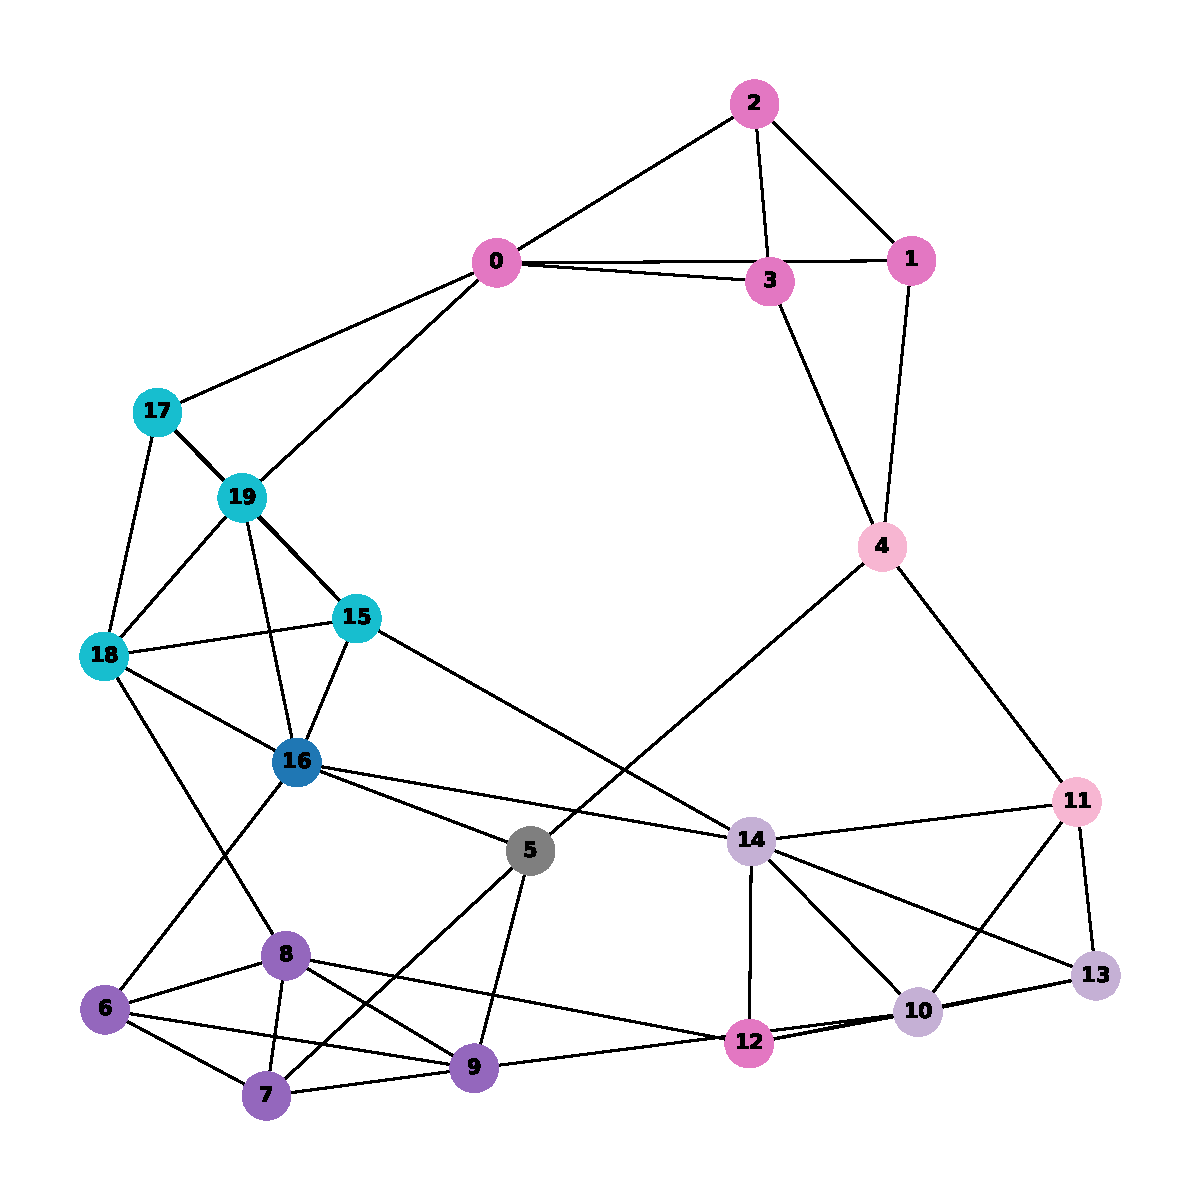
\includegraphics[width=0.6\linewidth]{iterations=6.pdf}
    \caption{7ο βήμα}
    \label{fig:it6}
  \end{subfigure}
  \begin{subfigure}{0.5\textwidth}
    \centering
    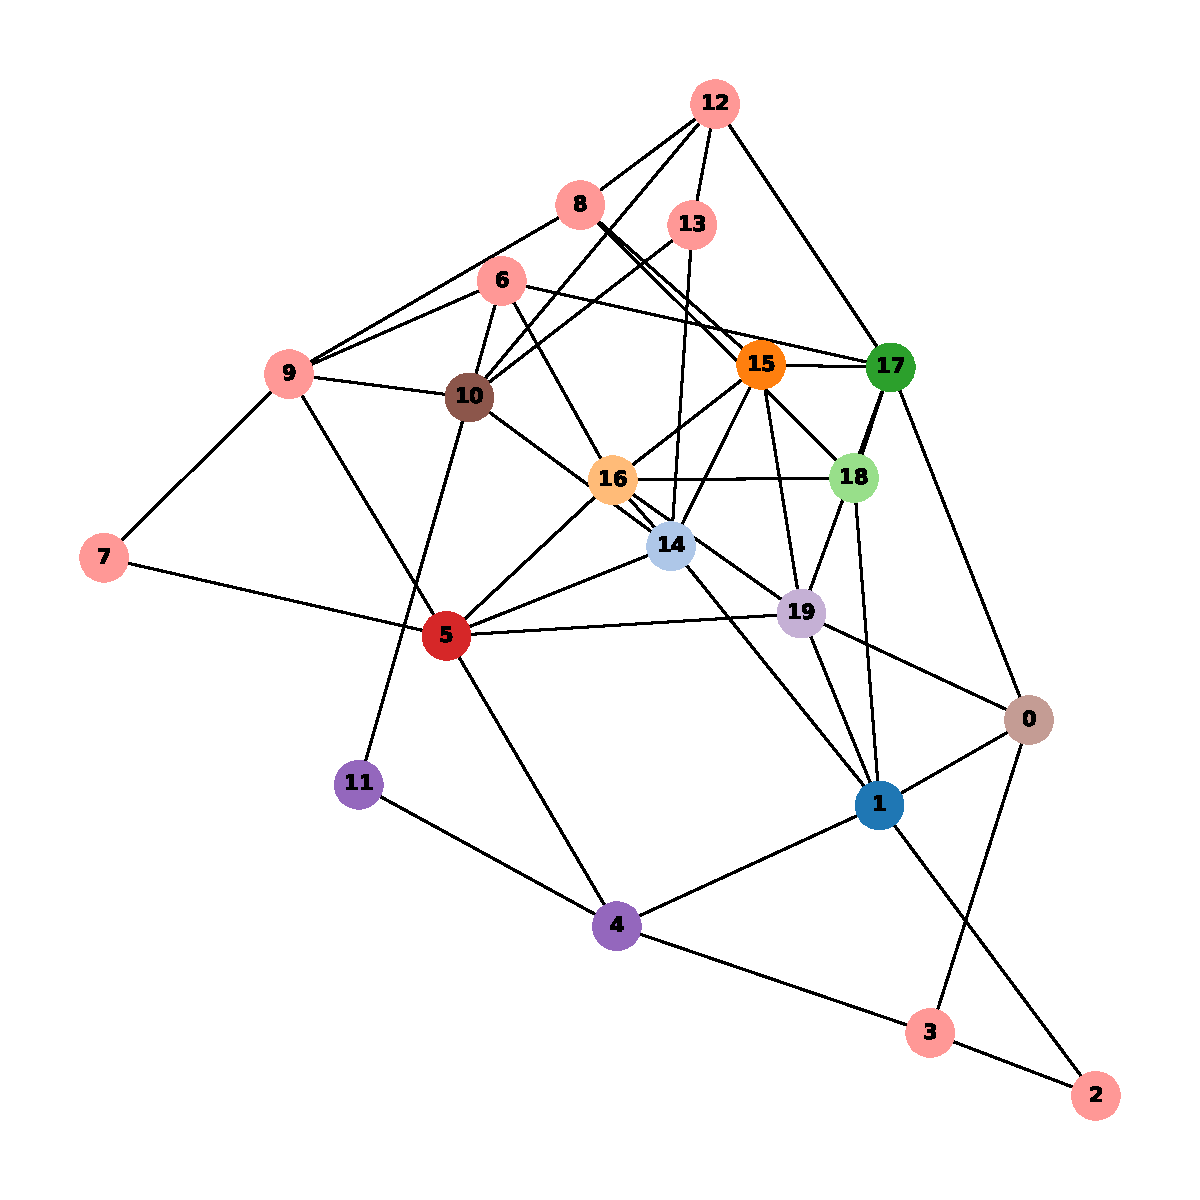
\includegraphics[width=0.6\linewidth]{iterations=15.pdf}
    \caption{16ο βήμα}
    \label{fig:it15}
  \end{subfigure}
  \caption{}
  \label{}
\end{figure}




Έπειτα σε κάθε βήμα αφαιρούμε μία ακμή (τυχαία) από το εσωτερικό των κοινοτήτων και την 
τοποθετούμε στο εξωτερικό τους (δηλαδή να ενώνει δύο διαφορετικές κοινότητες), έτσι 
\say{χαλάμε} σε κάθε βήμα την ποιότητα των κοινοτήτων. Για κάθε βήμα εκτιμούμε με τον 
αλγόριθμό μας τις κοινότητες και τις συγκρίνουμε με τις πραγματικές (\textlatin{Jaccard similarity}).

Στα σχήματα \ref{fig:it1}, \ref{fig:it6}, \ref{fig:it15} βλέπουμε τις εκτιμήσεις του 
αλγορίθμου για βήματα 2,7,16. Βλέπουμε ότι ο αλγόριθμος δεν έχει πολύ καλή απόδοση 
(ειδικά στο βήμα 2 όπου οι κοινότητες θα έπρεπε να είναι ξεκάθαρες), αλλά καταφέρνει 
να ανιχνεύσει κάποια δομή. Στο βήμα 16 όπου η δομή κοινοτήτων δεν είναι καθόλου ξεκάθαρη, 
τα αποτελέσματα είναι αρκετά κακά.

Στο σχήμα \ref{bench1} αποτυπώνουμε την απόδοση (\textlatin{Jaccard similarity})
του αλγορίθμου μας και την αντίστοιχη της \textlatin{modularity} για 20 βήματα.  
Για να εξαλειφθεί ο τυχόν θόρυβος από τις τυχαίες διαδικασίες πάρθηκε ο μέσος όρος 
για 100 ίδια πειράματα. 

Για τη \textlatin{modularity} χρησιμοποιήθηκε η συνάρτηση $greedy\_modularity\_communities$ της 
βιβλιοθήκης \textlatin{networkx}, η οποία λειτουργεί με τον αλγόριθμο των \en Clauset-Newman-Moore \gr 
\cite{Clauset:fastgreedy}\relax.
 
Η \textlatin{distance} έχει σαφώς χειρότερα αποτελέσματα.


\begin{figure}[H]
  \centering
  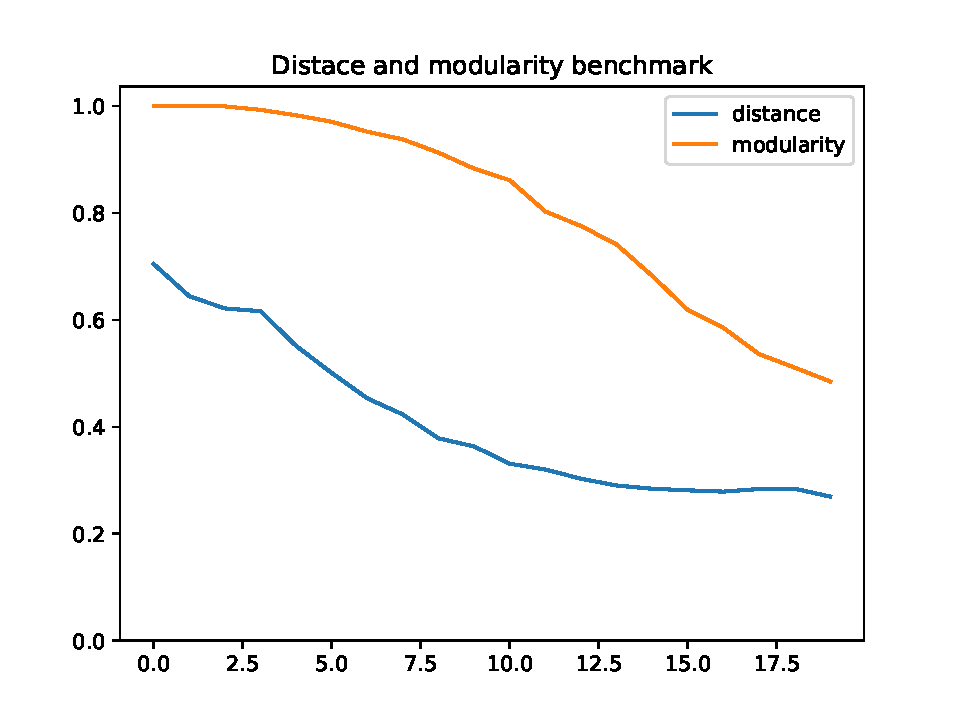
\includegraphics[width=0.5\linewidth]{benchmark.pdf}
  \caption{Μέση απόδοση με \textlatin{Jaccard similarity} των δύο μετρηκών. \\
  Στον οριζόντιο άξονα τα βήματα της διαδικασίας φθοράς του γράφου, στον κάθετο η απόδοση.}
  \label{bench1}
\end{figure}


\subsection{\textlatin{Newman}}

Για καλύτερα αποτελέσματα υλοποιήθηκε ο αλγόριθμος που προτάθηκε από τον \textlatin{Newman} 
\cite{Newman}\relax. 

Ο αγλόριθμος αυτός προτάθηκε για τη μεγιστοποίηση της \en modularity, \gr αλλά μπορεί με τις κατάλληλες τροποποιήσεις να χρησιμοποιηθεί και εδώ.

Ξεκινάμε με μια κοινότητα για κάθε κόμβο αλλά αυτή τη φορά ενώνουμε διαδοχικά \emph{τις κοινότητες} οι οποίες θα έχουν μέγιστη αύξηση του $Q$. Μετά από $|V|-1$ συνδέσεις
θα έχει μείνει μόνο μία κοινότητα, όποτε απαιτούνται το πολύ $|V|-1$ συνδέσεις. 

Στην ταχύτητα βοηθάει η παρατήρηση ότι δε χρειάζεται να υπολογίζεται συνέχεια η τιμή της $Q_d$ αλλά μόνο η διαφορά $\Delta Q_d(c_i,c_j)$ της $Q_d$ αν συνενώσουμε τις 
κοινότητες $c_i$ και $c_j$. 


Αναλυτικά:

Έστω ότι έχω κοινότητες $C = {c_1,..,c_n}$ και συνενώνω τις κοινότητες $c_i,c_j \in C$ ώστε να αποκτήσω
στο επόμενο βήμα κοινότητες $C'$. Έστω επίσης ότι $Q_d$ είναι η τιμή της \textlatin{distance quality}
στις κοινότητες $C$, ενώ $Q_d'$ στις $C'$. 



Για ευκολία συμβολίζω: 
\[ I(c) = (1 - \gamma)\overline{ D_V(c) } - \gamma D_V(c) \]
και,
\[ J(i,j) = (1-\gamma) \overline{ D_V(i,j)} - \gamma D_V(i,j) \]
τότε,
\[ Q_d = \sum_{c \in C} I(c) =\sum_{c \in C} \sum_{i,j \in c} J(i,j) \]
Έχουμε:
\[ Q_d  = \sum_{c \in C} I(c) =  \sum_{c \in C \setminus c_i,c_j}[I(c)] + I(c_i) + I(c_j) \Leftrightarrow\]
\[ Q_d = \sum_{c \in C \setminus c_i,c_j}[I(c)] + \sum_{i,j \in c_i}J(i,j) + \sum_{i,j \in c_j}J(i,j)  \]
καi,
\[ Q_d' = \sum_{c \in C'} I(c) =  \sum_{c \in C' \setminus (c_i \cup c_j)}[I(c)] + I(c_i \cup c_j) \Leftrightarrow \]
\[ Q_d' =  \sum_{c \in C \setminus c_i,c_j}[I(c)] + \sum_{i,j \in c_i \cup c_j} J(i,j) \]



Από τα παραπάνω είναι φανερό ότι:
\[   \Delta Q = Q_d' - Q_d = 2 \sum_{i \in c_i, j \in c_j} J(i,j) \Leftrightarrow \]
\[ \Delta Q = 2 \sum_{i \in c_i, j \in c_j} (1-\gamma) \overline{ D_V(i,j)} - \gamma D_V(i,j) \]

\bigskip

Επιπλέον, όταν ενώνονται δύο κοινότητες $c_i,c_j$, έστω στην $c_j$, τότε για κάθε 
άλλη κοινότητα $c_k$ η τιμή $\Delta Q_{jk}$ μεταβέλεται ως εξίς:

\[ \Delta Q_{jk}' = 2 \sum_{i \in c_i \cup c_j, j \in c_k} J(i,j) = 2 \sum_{i \in c_i, j \in c_k} J(i,j) + 2 \sum_{i \in c_j, j \in c_k} J(i,j) = \Delta Q_{ik} + \Delta Q_{jk}\]


Τώρα είμαστε σε θέση να ορίσουμε τον αλγόριθμο:

Διατηρούμε έναν πίνακα $\Delta Q$ που θα περιέχει για κάθε δύο κοινότητες $c_i,c_j$ 
τη τιμή $\Delta Q_{ij}$. Για την αρχική περίπτωση όπου κάθε κόμβος $v$ έχει δική του 
κοινότητα $c=\{v\}$: 
\begin{equation}   \label{init_dq}
  \Delta Q_{ik} = 2 \cdot [(1-\gamma)\overline{ D_V(c_i,c_j)} - \gamma  D_V(c_i,c_j)   ]
\end{equation}



\begin{enumerate}
  \item Υπολογίζουμε τις απαραίτητες ποσότητες και τις αποθηκεύουμε \\ ($D_V(i,j), \ d_k(i), \ m_G(k), \ Pr[i,j,k],  \ \overline{D_V(i,j)},diam(G)$). 
  \item Αρχικοποιούμε κάθε κόμβο σε δική του κοινότητα.
  \item Αρχικοποιούμε τον πίνακα $\Delta Q$ σύμφωνα με την εξίσωση \ref{init_dq}. 
  \item Βρίσκουμε το μέγιστο στοιχείο του πίνακα $\Delta Q$. Αυτό το στοιχείο μας 
  δίνει ποιές κοινότητες θα δώσουν τη μέγιστη διαφορά στην $Q_d$ αν ενωθούν.
  \item Αν το $max \Delta Q_{ij}$ που βρήκαμε είναι θετικό, ενώνουμε τις κοινότητες 
  $c_i, c_j$ στην $c_j$, ανανεώνουμε τα στοιχεία του πίνακα $\Delta Q$ ως εξίς:
  \[ \Delta Q_{jk} = \Delta Q_{kj} = \Delta Q_{ik} + \Delta Q_{jk}, \ \ \ \ \Delta Q_{ik} = \Delta Q_{ki} = -\infty \]
  και επιστρέφουμε στο βήμα 4. 
  \item Αν το $max \Delta Q_{ij}$ που βρήκαμε είναι αρνητικό, τότε τερματίζουμε τον αλγόριθμο
  και επιστρέφουμε τις κοινότητες όπως είναι σε αυτό το βήμα. 
\end{enumerate}





Σύμφωνα με την έρευνα των \en Clauset-Newman-Moore \gr \cite{Clauset:fastgreedy},
από το βήμα όπου το $max \Delta Q$ γίνει για πρώτη φορά αρνητικό και μετέπειτα, θα 
συνεχίσει να είναι αρνητικό. Δηλαδή η $Q_d$ θα μειώνεται σταδιακά. Επομένως μόλις φτάσουμε 
σε αυτό το στάδιο μπορούμε να τερματίσουμε τον αλγόριθμο, αφού βρήκαμε το μέγιστο. 

Αυτός ο αλγόριθμος είναι ήδη σημαντικά πιο γρήγορος από τον προηγούμενο, αφού το εσωτερικό 
της λούπας πλέον απλοποιείται στην εύρεση μέγιστου στοιχείου ενός πίνακα. Τα υπόλοιπα είναι 
μόνο προσθέσεις, αναθέσεις πινάκων και έλεγχοι, όλες διεργασίες 
σταθερού χρόνου. Επίσης στον αλγόριθμο αυτόν δεν χρειάζεται να υπολογιστεί η $Q_d$ 
αναλυτικά, αλλά μόνο τα αρχικά $\Delta Q$ που είναι σημαντικά απλούστερα.

Μια άμεση βελτίωση που θα μπορούσε να γίνει \cite{Clauset:fastgreedy} είναι να τοποθετούμε 
τα $\Delta Q_{ij}$ σε μια σωρό μεγίστων, ώστε να αποφευχθεί το $O(|V|^2)$ της εύρεσης 
μεγίστου στον πίνακα σε $O(log|V|)$. Όμως αυτό δε το υλοποίησα στο πλαίσιο της παρούσης 
εργασίας.

\subsubsection{Απόδοση}


Στα σχήματα \ref{new_1}, \ref{new_2} φαίνονται τα αποτελέσματα του συγκεκριμένου αλγόριθμου 
με τις ίδιες τεχνικές όπως προηγουμένως. 
Ο αλγόριθμος \textlatin{Newman} φαίνεται να έχει ίσως χειρότερα (ή αντίστοιχα) αποτελέσματα από/με τον 
προηγούμενο, το οποίο είναι αναμενόμενο αφού ενώνει κάθε φορά ολόκληρες κοινότητες 
αντί για μεμονομένους κόμβους και έτσι μια λάθος ένωση στην αρχή, διαδίδεται και πολλαπλασιάζεται.

Το πλεονέκτιμά του είναι η ταχύτητα. 



\begin{figure}[H]
  \begin{subfigure}{0.5\textwidth}
    \centering
    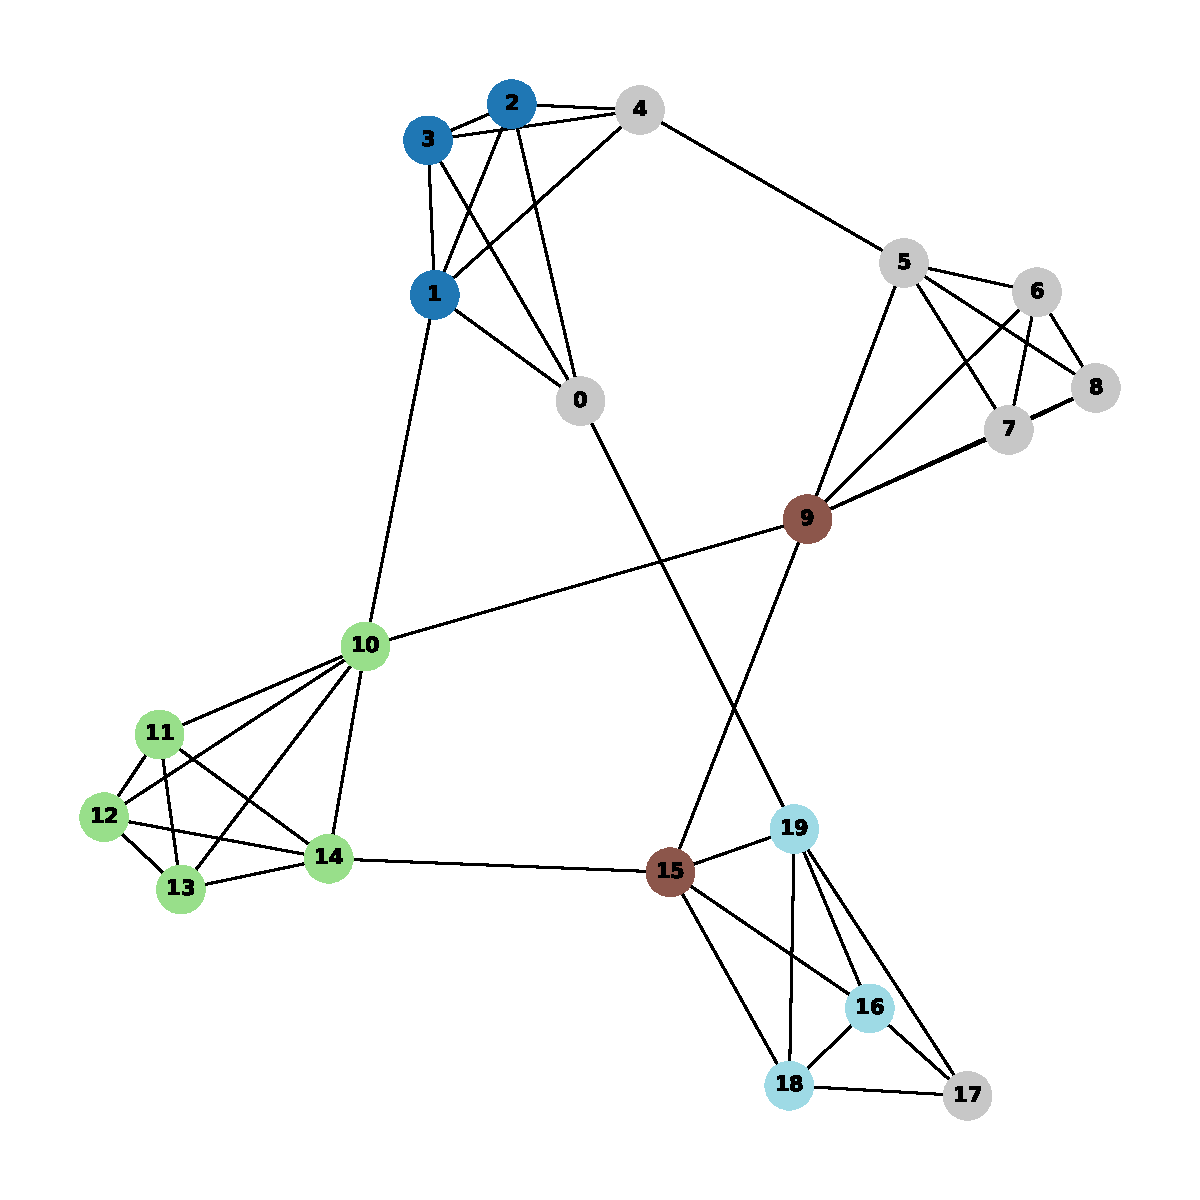
\includegraphics[width=0.6\linewidth]{iterations=1newman.pdf}
    \caption{Αποτελέσματα αλγορίθμου \textlatin{Newman} στο 2ο βήμα. ($\gamma=0.15$)}
    \label{fig:it1new}
  \end{subfigure}
  \begin{subfigure}{0.5\textwidth}
    \centering
    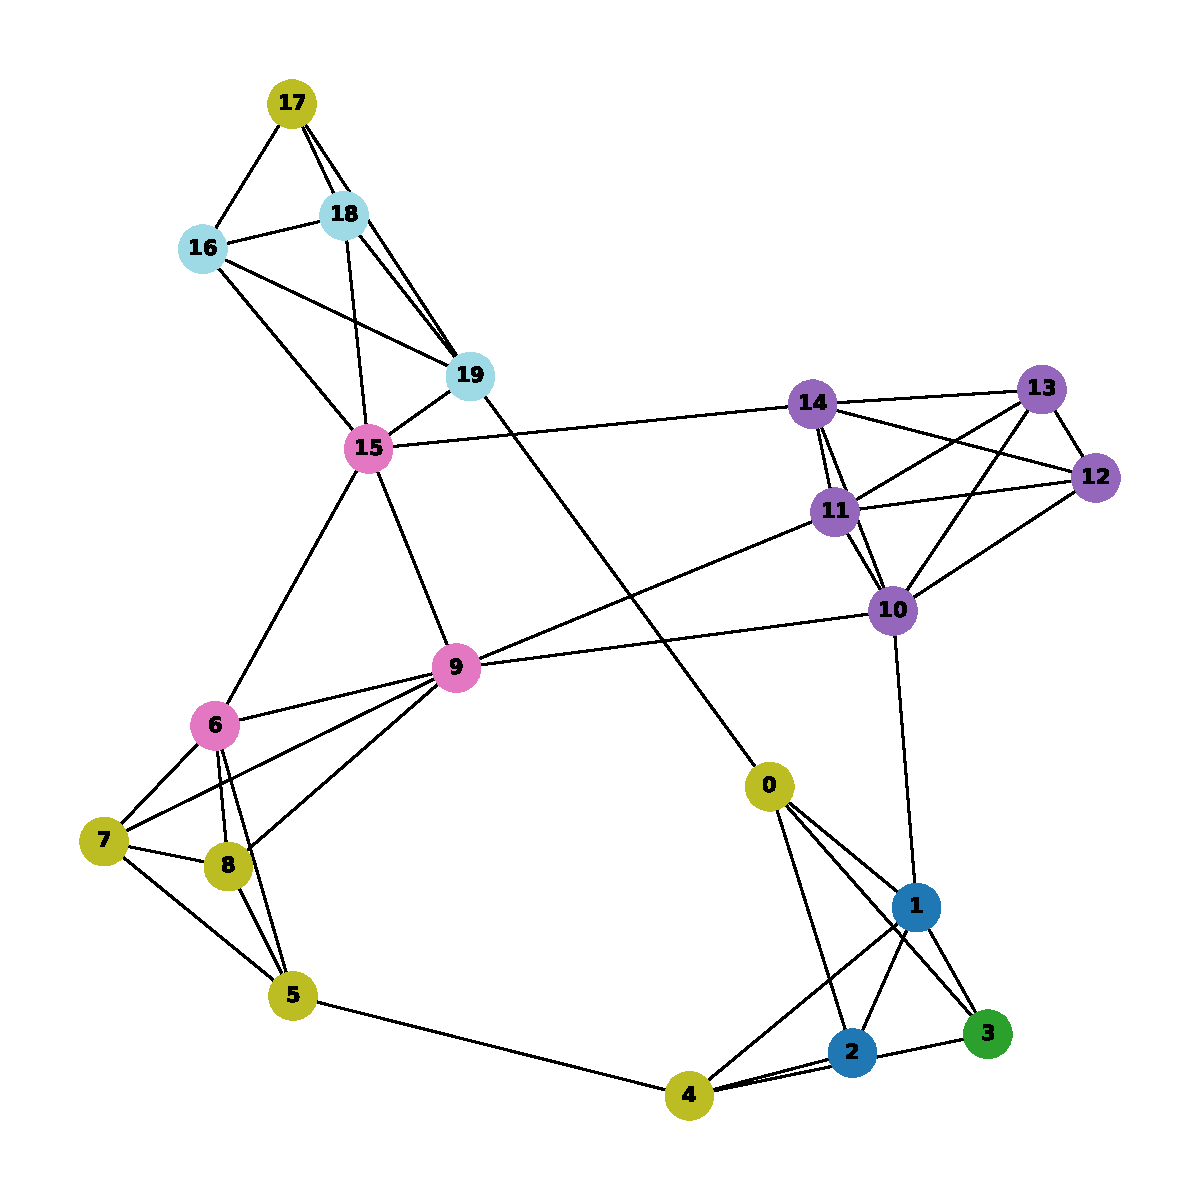
\includegraphics[width=0.6\linewidth]{iterations=3newman.pdf}
    \caption{Αποτελέσματα αλγορίθμου \textlatin{Newman} στο 4ο βήμα. ($\gamma = 0.15$)}
    \label{fig:it3new}
  \end{subfigure}
  \caption{}
  \label{new_1}
\end{figure}




\begin{figure}[H]
  \begin{subfigure}{0.5\textwidth}
    \centering
    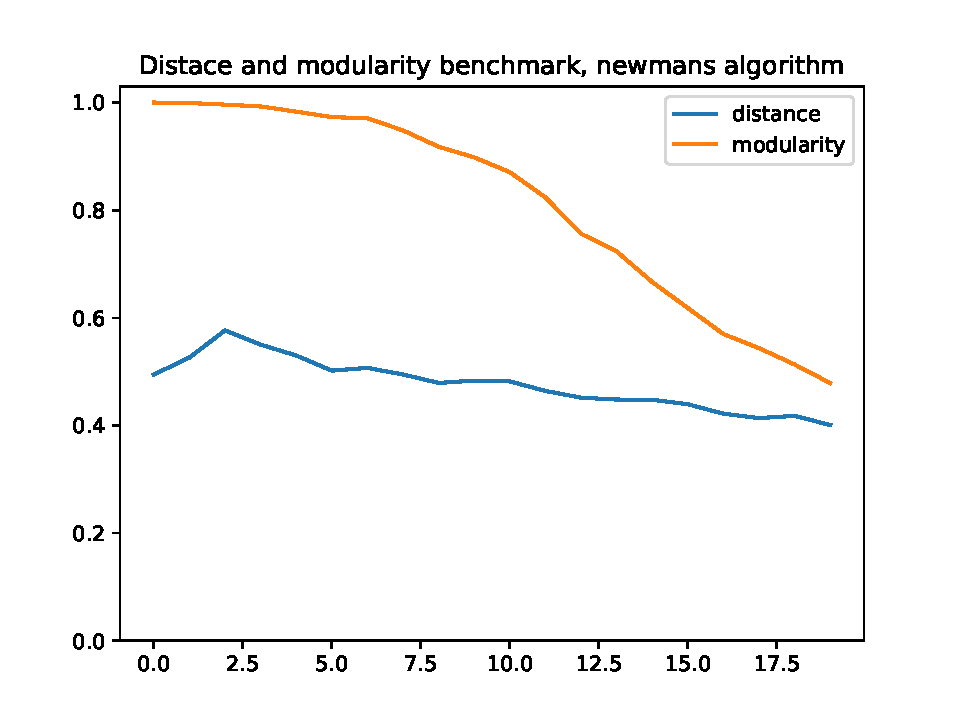
\includegraphics[width=0.8\linewidth]{benchmark_newman_gamma=0.01.pdf}
    \caption{$\gamma = 0.01$}
    \label{fig:bench0.01new}
  \end{subfigure}
  \begin{subfigure}{0.5\textwidth}
    \centering
    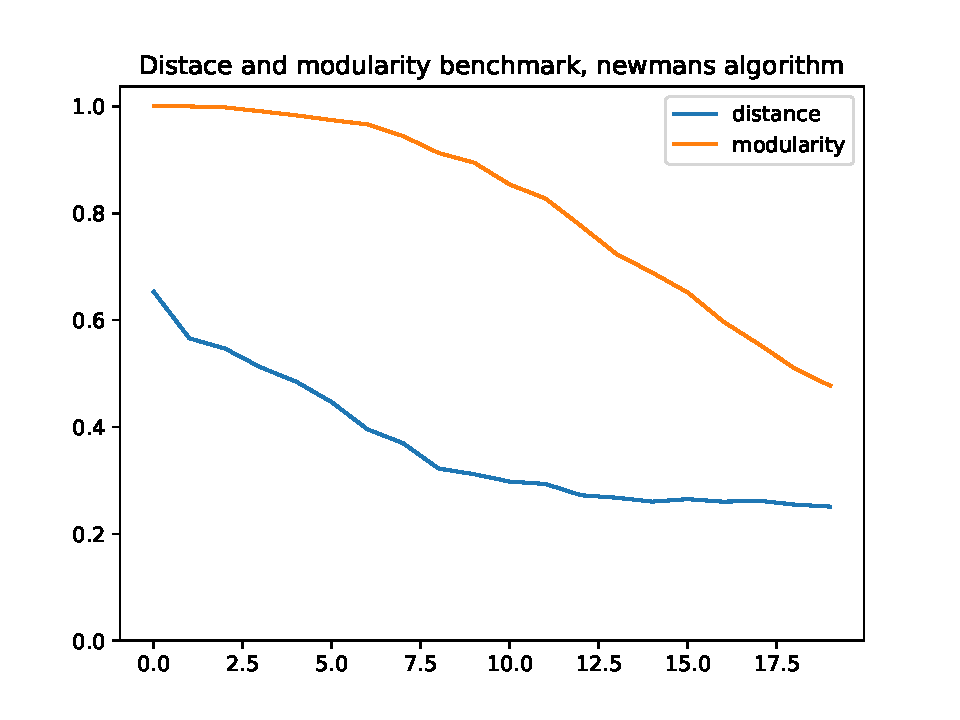
\includegraphics[width=0.8\linewidth]{benchmark_newman_gamma=0.02.pdf}
    \caption{$\gamma = 0.02$}
    \label{fig:bench0.02new}
  \end{subfigure}
  \caption{Μέση απόδοση με χρήση \textlatin{Jaccard similarity}, στη \textlatin{distance}
  χρησιμοποιήθηκε αλγόριθμος \textlatin{Newman}.}
  \label{new_2}
\end{figure}





\subsection{Χρονική πολυπλοκότητα και σύγκριση}



Για τους δύο αλγορίθμους το πρώτο στάδιο είναι παρόμοιο (υπολογισμός απαραίτητων ποσοτήτων), δεν αναφέρω την χρονική πολυπλοκότητα
του, μιας και δεν βρήκα τις χρονικές πολυπλοκότητες των συναρτήσεων της βιβλιοθήκης
$networkx$ που χρησιμοποίησα.

Ούτως ή άλλως, όμως, το αργό στάδιο είναι το δεύτερο, αυτό της βελτιστοποίησης της 
δομής κοινοτήτων. 

\begin{itemize}
  \item Στον πρώτο αλγόριθμο τρέχουμε για κάθε κόμβο και κάθε γείτονα του, την δεύτερη
  φάση του υπολογισμού της $Q_d$ (βλ. \ref{ylop}), η οποία είναι $O(|V|^2)$. 
  Επομένως έχουμε πολυπλοκότητα χειρότερης περίπτωσης: $O(|V|^4)$. 
  Αυτή η διαδικασία όμως γίνεται όσες φορές χρειάζεται ώστε να μην βελτιώνεται άλλο 
  η $Q_d$. Στον κώδικα έχει δωθεί ένα άνω φράγμα επαναλύψεων (\textlatin{max iterations} = $maxit$),
  έτσι η πολυπλοκότητα χειρότερης περίπτωσης είναι συνολικά $O(maxit \cdot |V|^4)$,
  όπου $|V|$ το πλήθος των κόμβων.


  \item Στον αλγόριθμο $Newman$ το εσωτερικό της λούπας, όπως ήδη αναφέρθηκε, είναι 
  $O(|V|^2)$ για την εύρεση του μέγιστου στοιχείου του πίνακα $\Delta Q$ (το οποίο μπορεί 
  και να βελτιωθεί με σωρό μεγίστων). Η λούπα επαναλαμβάνεται το πολύ $|V|-1$
  φορές, και έτσι έχουμε συνολοκή πολυπλοκότητα χειρότερης περίπτωσης: $O(|V|^3)$.


\end{itemize}





\subsection{Επιρροή της τιμής $\gamma$}  \label{gamma}


\begin{figure}[H]
  \begin{subfigure}{0.5\textwidth}
    \centering
    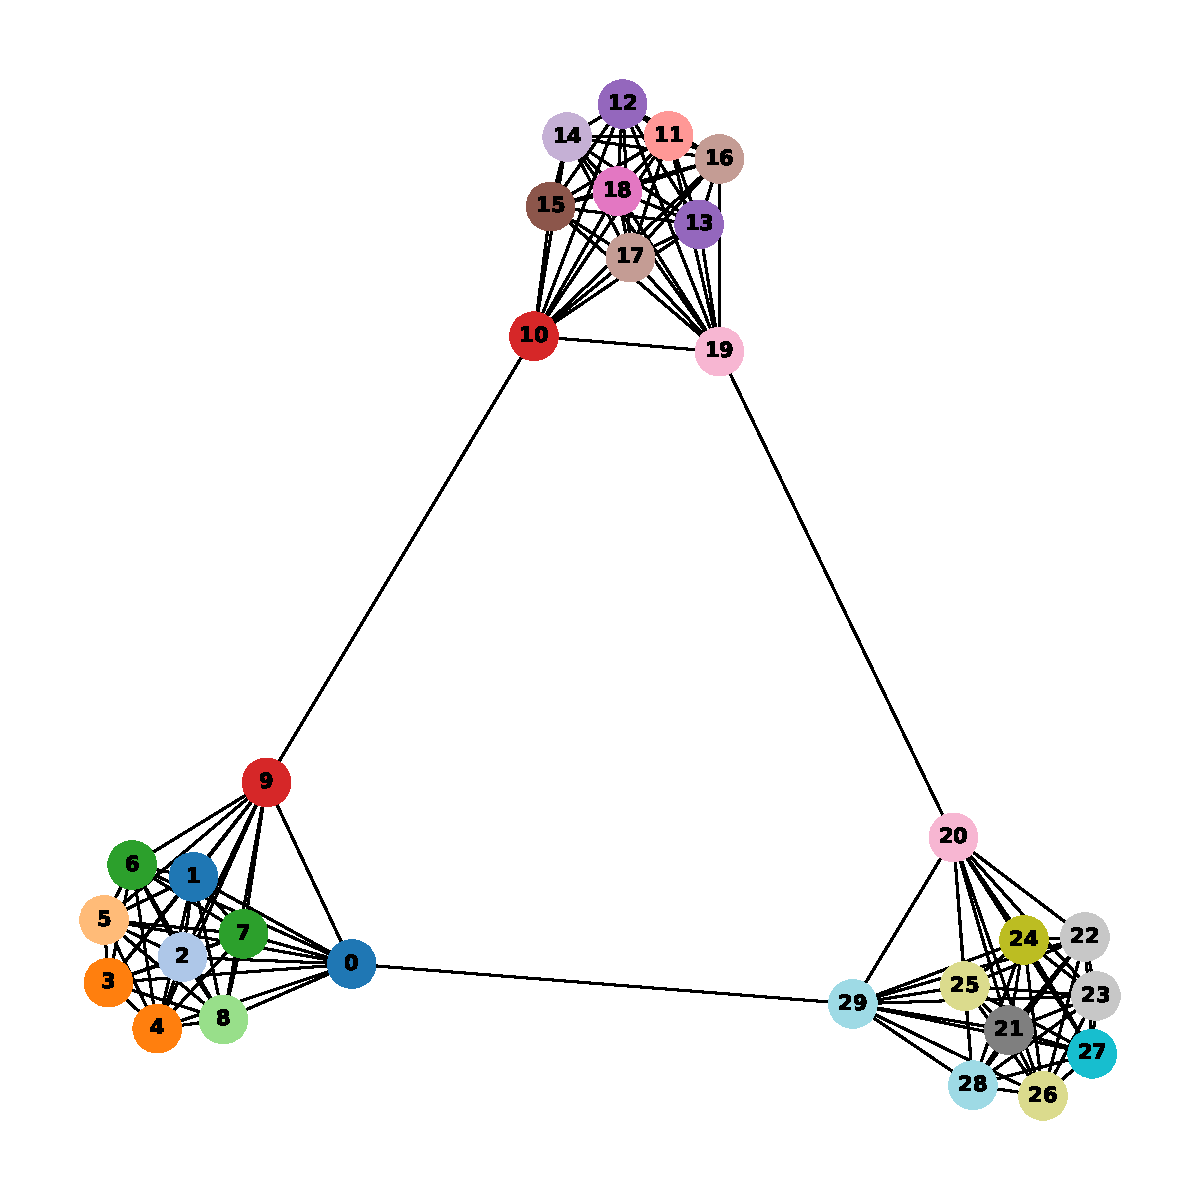
\includegraphics[width=0.8\linewidth]{gammachange3,10gamma=0.02.pdf}
    \caption{$\gamma = 0.02$}
    \label{g1}
  \end{subfigure}
  \begin{subfigure}{0.5\textwidth}
    \centering
    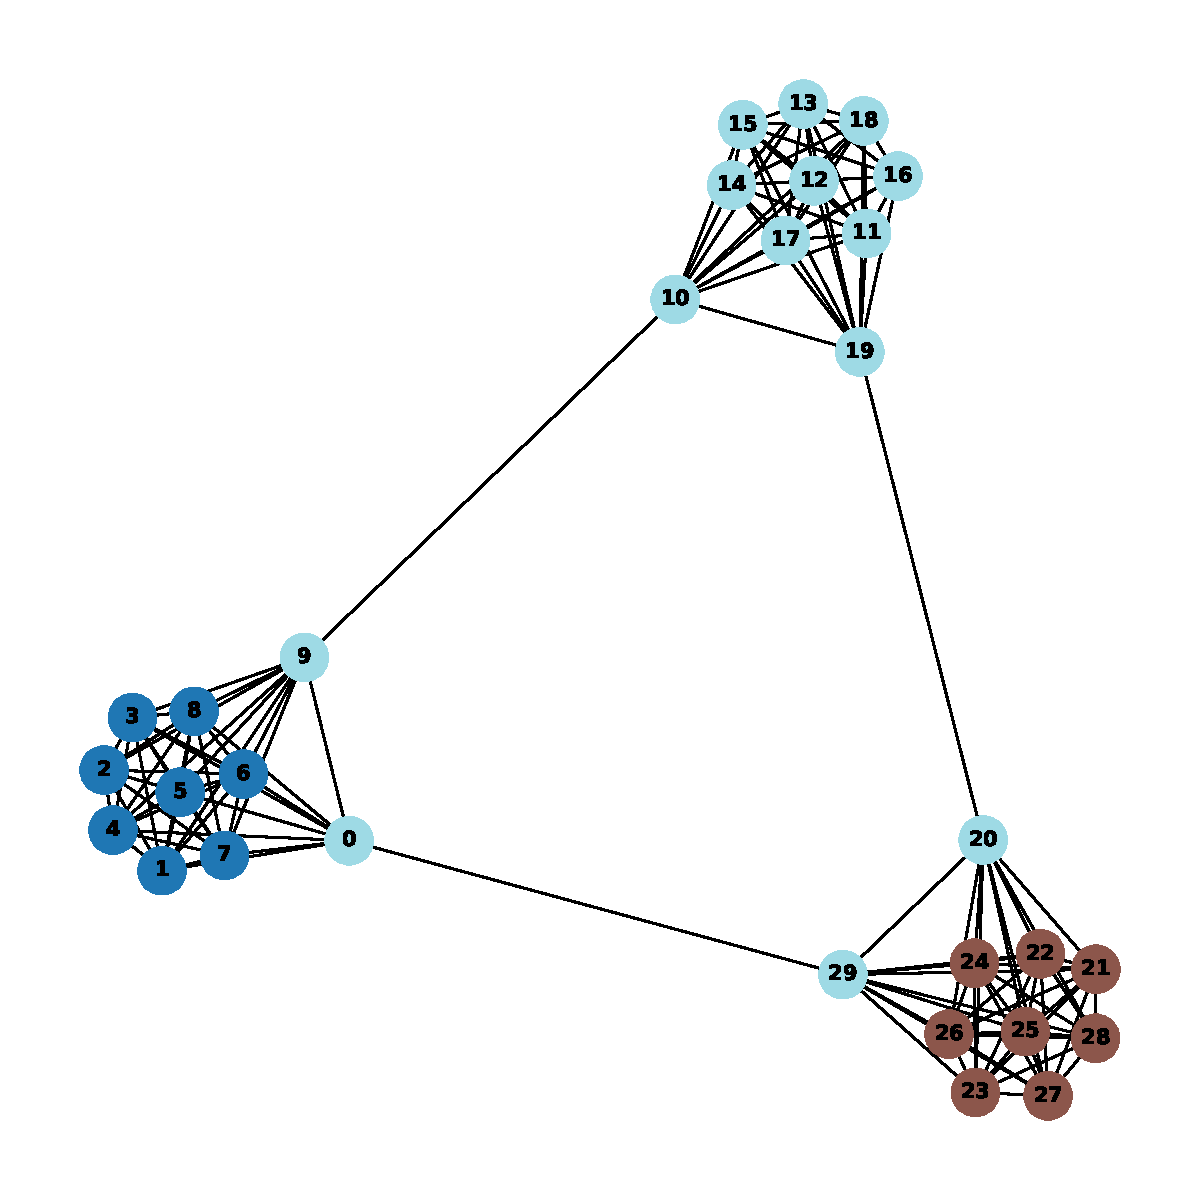
\includegraphics[width=0.8\linewidth]{gammachange3,10gamma=0.003.pdf}
    \caption{$\gamma = 0.03$}
    \label{g2}
  \end{subfigure}

  \vfill

  \begin{subfigure}{0.5\textwidth}
    \centering
    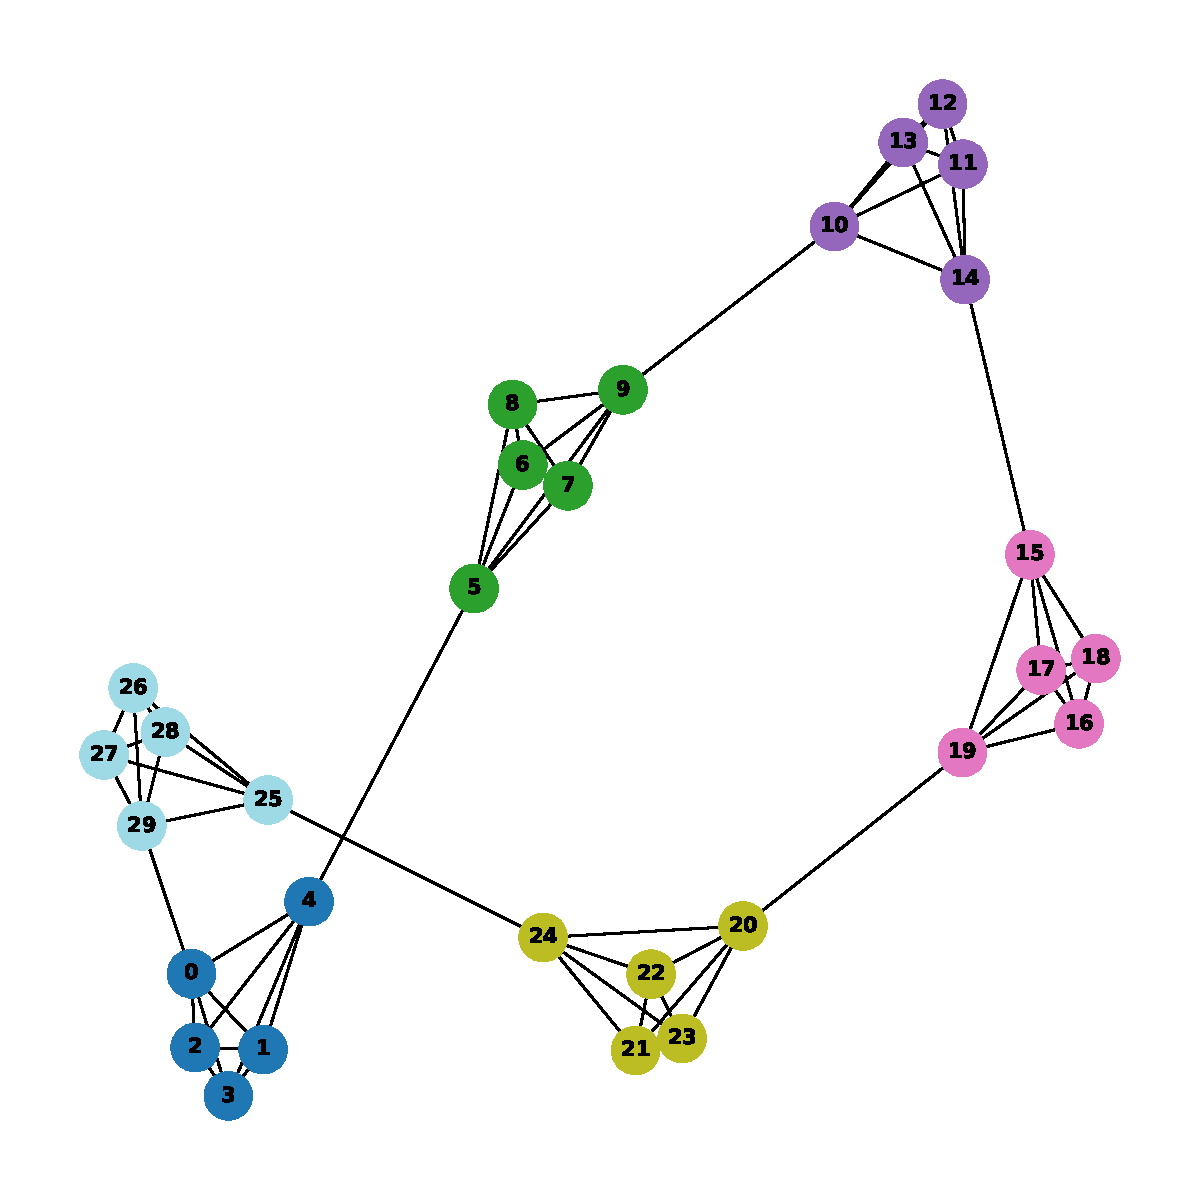
\includegraphics[width=0.8\linewidth]{gammachange6,5gamma=0.02.pdf}
    \caption{$\gamma = 0.02$}
    \label{g3}
  \end{subfigure}
  \begin{subfigure}{0.5\textwidth}
    \centering
    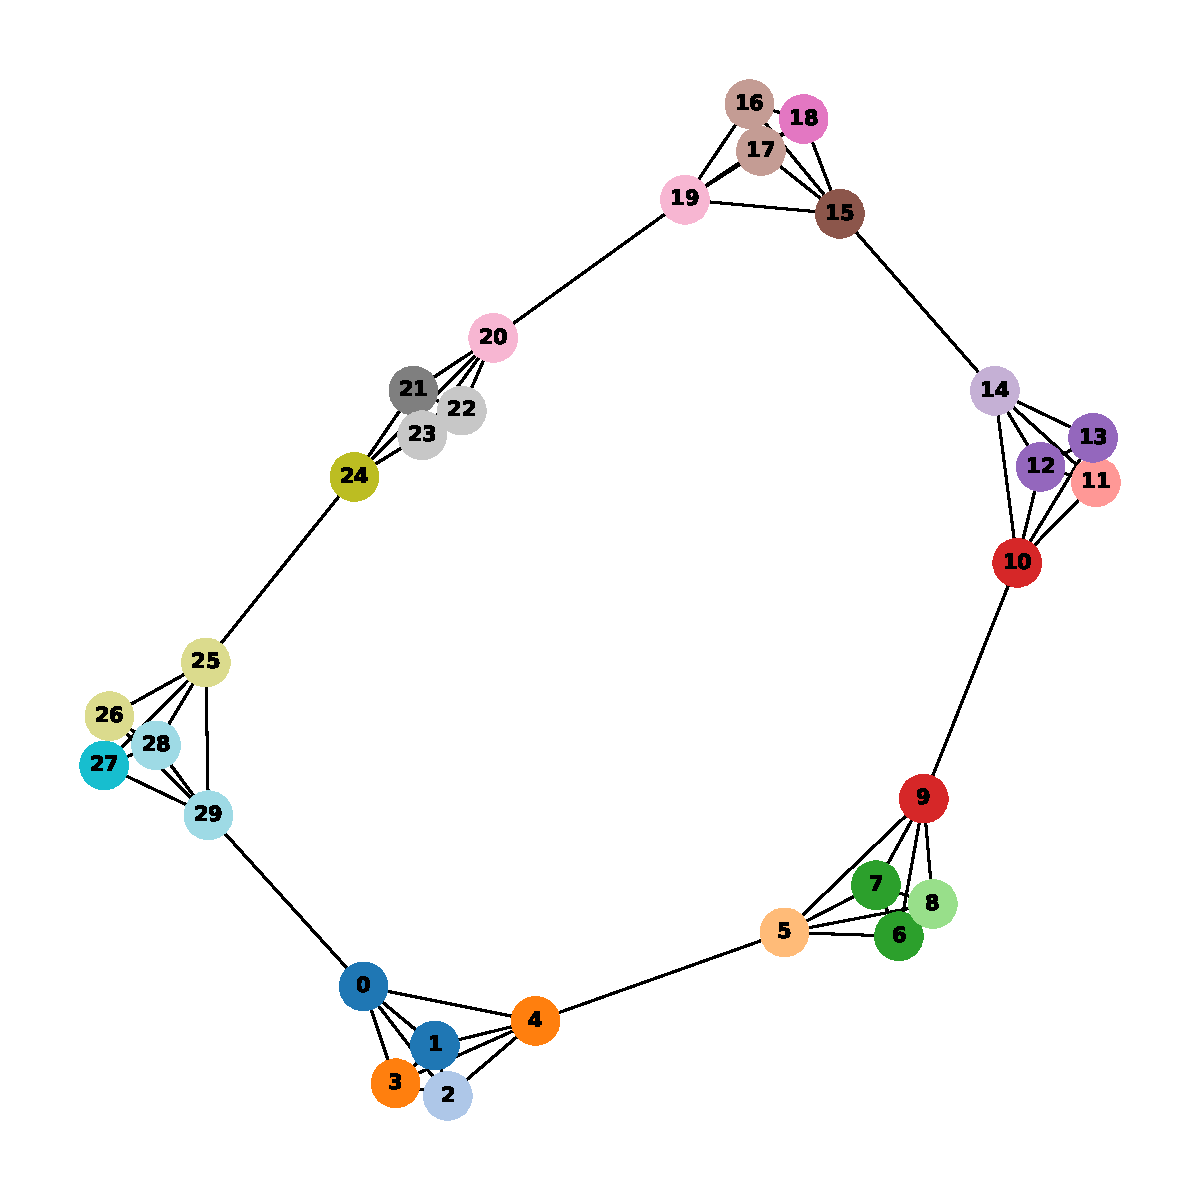
\includegraphics[width=0.8\linewidth]{gammachange6,5gamma=0.04.pdf}
    \caption{$\gamma = 0.03$}
    \label{g4}
  \end{subfigure}


  \caption{Αποτελέσματα γράφων για διαφορετικές τιμές του $\gamma$
  με τον αλγόριθμο \textlatin{Newman}.}
  \label{gamma_tests}
\end{figure}







Στο σχήμα \ref{gamma_tests} φαίνοται τα αποτελέσματα δύο γράφων για διαφορετικές τιμές
του $\gamma$. Βλέπουμε ότι ο γράφος στο \ref{g1} για $\gamma = 0.02$ δεν έχει καλά 
αποτελέσματα, ενώ στο \ref{g2} για $\gamma = 0.003$ έχει πολύ καλύτερα. Το αντίθετο 
ισχύει για το γράφο των \ref{g3}, \ref{g4}, όπου για $\gamma = 0.02$ έχει άρτια αποτελέσματα.

Έιναι ξεκάθαρη η επιρροή του $\gamma$ όμως η βέλτιστη τιμή του είναι διαφορετική 
σε κάθε γράφο. Έτσι παρουσιάζεται το ερώτημα: \emph{μπορούμε να εκτιμήσουμε τη 
βέλτιστη τιμή του $\gamma$?}

% plots of same size different cluster size




Μια παρατήρηση που κάνουμε εξ αρχής είναι ότι η βέλτιστη τιμή του $\gamma$ φαίνεται 
να μικραίνει όσο μεγαλώνει το μέγεθος των κοινοτήτων. Έτσι δοκιμάστηκε να βρεθεί 
η σχέση τους, εάν αυτή υπάρχει: 
Δημιουργήθηκαν τυχαίοι γράφοι με την τεχνική που παρουσιάστηκε και προηγουμένως 
για διαφορετικά μεγέθη των κοινοτήτων (πλήρεις υπογράφοι). Για κάθε κάθε τέτοιο 
γράφο δοκιμάστηκαν πολλές τιμές $\gamma$ και βρέθηκε η βέλτιστη από αυτές. 
Βρέθηκε ξεκάθαρη εξάρτηση της βέλτιστης τιμής $\gamma$ και του μεγέθους κοινότητας.




Στο σχήμα \ref{optimal_gamma} απεικονίζεται η εξάρτηση αυτή για μεγέθη κοινοτήτων 
απο 1 μέχρι 50 κόμβους. Παρατηρούμε εκθετική μείωση, οπότε δοκιμάστηκε να προσαρμωστεί 
η καμπύλη $c e^{- \lambda x}$ (δηλαδή να βρεθούν σταθερές $c, \lambda$) στα δεδομένα.
Χρησιμοποιήθηκε η συνάρτηση $scipy.optimise.curve\_fit$.

Το αποτέλεσμα φαίνεται στο σχήμα \ref{optimal_gamma_approx} για $c = 0.1616558536042243, \lambda = 0.4500547630497226$.


Έτσι δημιουργήθηκε μια παραλλαγή του αλγορίθμου $Newman$, όπου αυτή τη φορά 
το $\gamma$ δε δίνεται ως είσοδος, αλλά υπολογίζεται με την σχέση $ce^{-\lambda x}$,
όπου $x$ το αναμενόμενο μέγεθος κοινοτήτων.

Αποτελέσματα της μεθόδου αυτής φαίνονται στο σχήμα \ref{auto_cluster_size}.
Στα παραδείγματα \ref{9a}, \ref{9b} κατάφερε με ακρίβεια να αναγνωρίσει 
τις κοινότητες, όμως στο \ref{9c} απέτυχε. Ίσως με περισσότερα δεδομένα 
να μπορούσε να εκτιμηθεί καλύτερα η καμπύλη της συσχέτησης του βέλτιστου $\gamma$
και να είχαμε καλύτερα αποτελέσματα. 




\begin{figure}[H]
  \begin{subfigure}{0.5\textwidth}
    \centering
    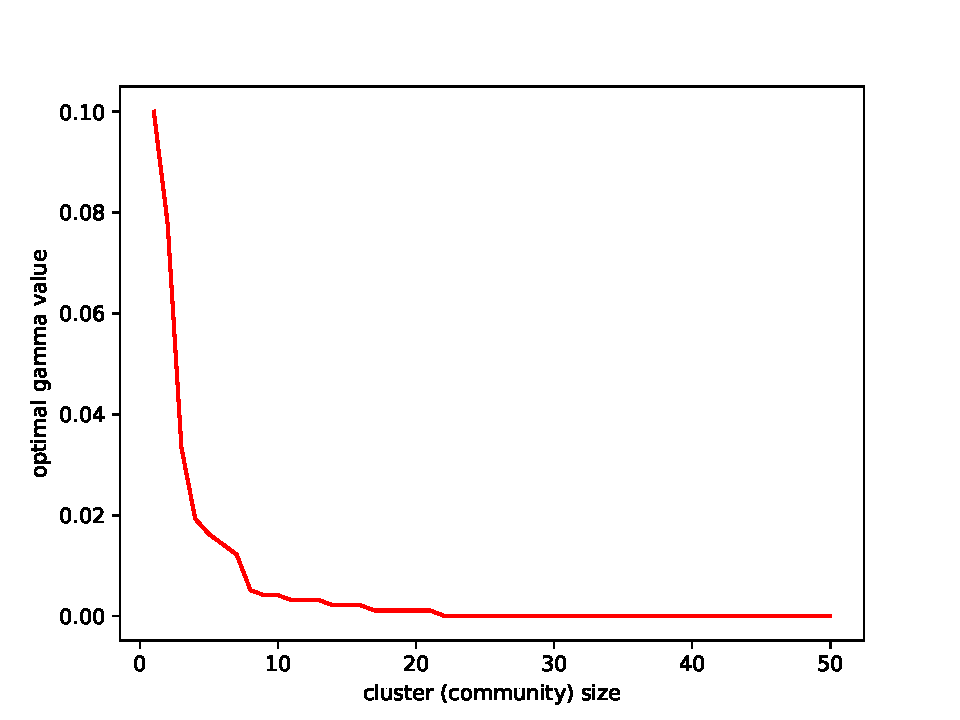
\includegraphics[width=0.9\linewidth]{gamma_wrt_cluster_nodes.pdf}
    \caption{Συσχέτηση βέλτιστου $\gamma$ ως προς μέγεθος κοινοτήτων}
    \label{optimal_gamma}
  \end{subfigure}
  \begin{subfigure}{0.5\textwidth}
    \centering
    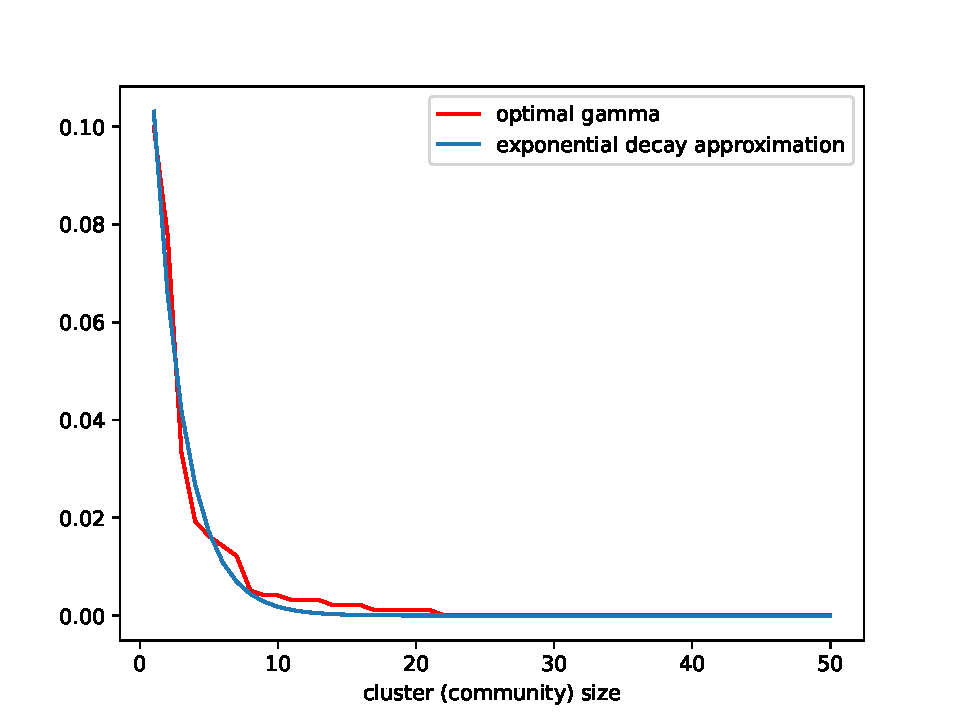
\includegraphics[width=0.9\linewidth]{gammas_approximation.pdf}
    \caption{Εκτίμηση της συσχέτησης. $c \approx 0.16, \lambda \approx 0.45$}
    \label{optimal_gamma_approx}
  \end{subfigure}

  \caption{}
  \label{}
\end{figure}




\begin{figure}[h]
  \centering
  \begin{subfigure}{0.3\textwidth}
      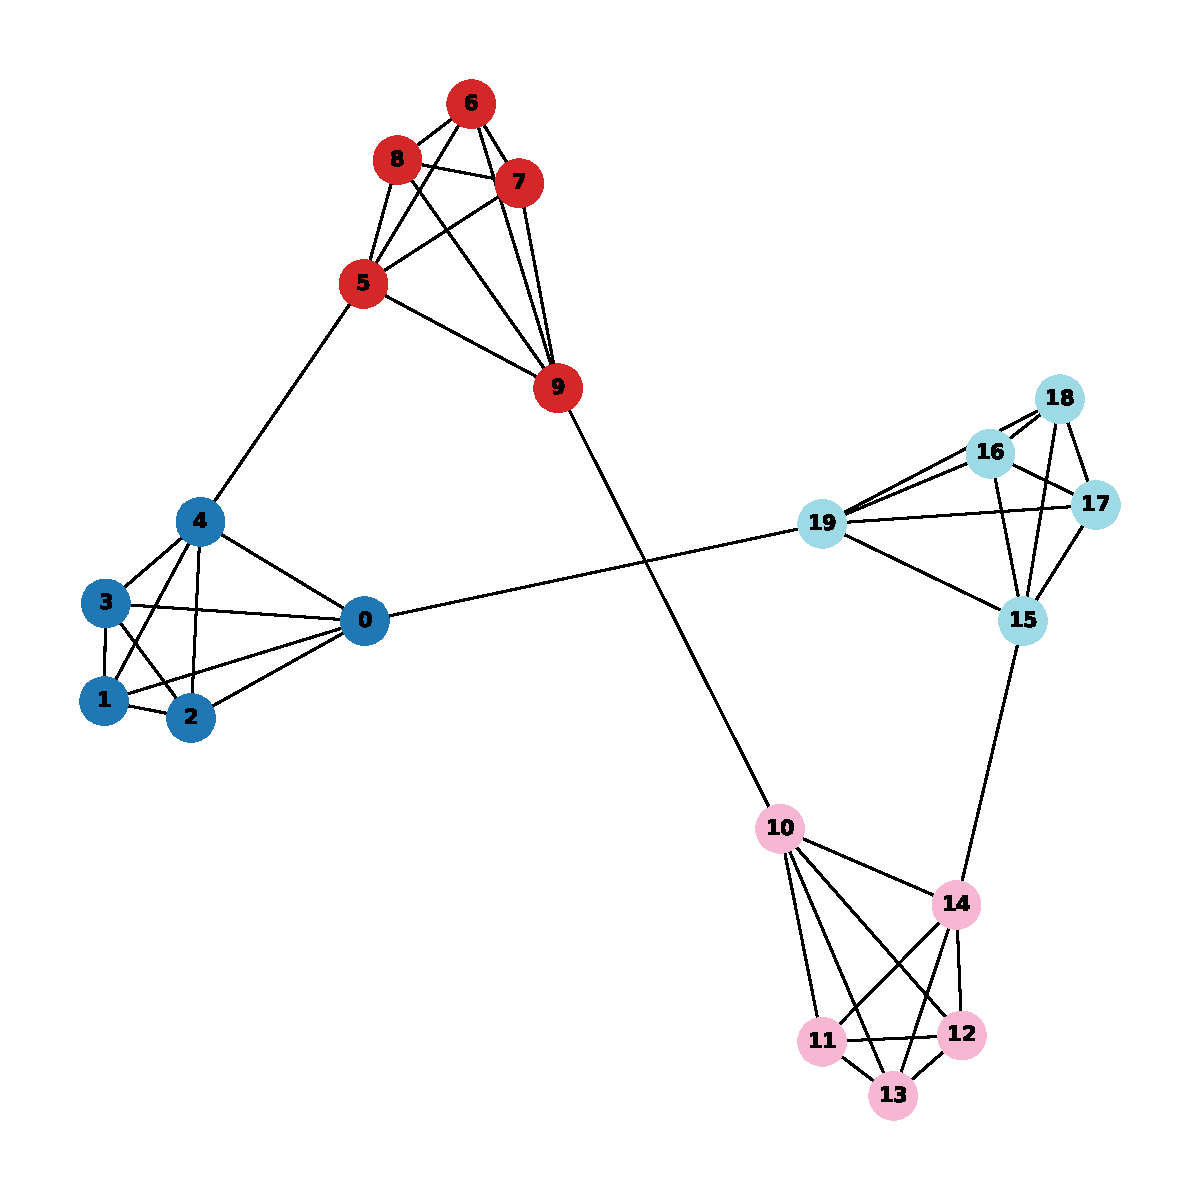
\includegraphics[width=\textwidth]{cluster_4,5newman_auto.pdf}
      \caption{4 κοινότητες από 5 κόμβους.}
      \label{9a}
  \end{subfigure}
  \begin{subfigure}{0.3\textwidth}
      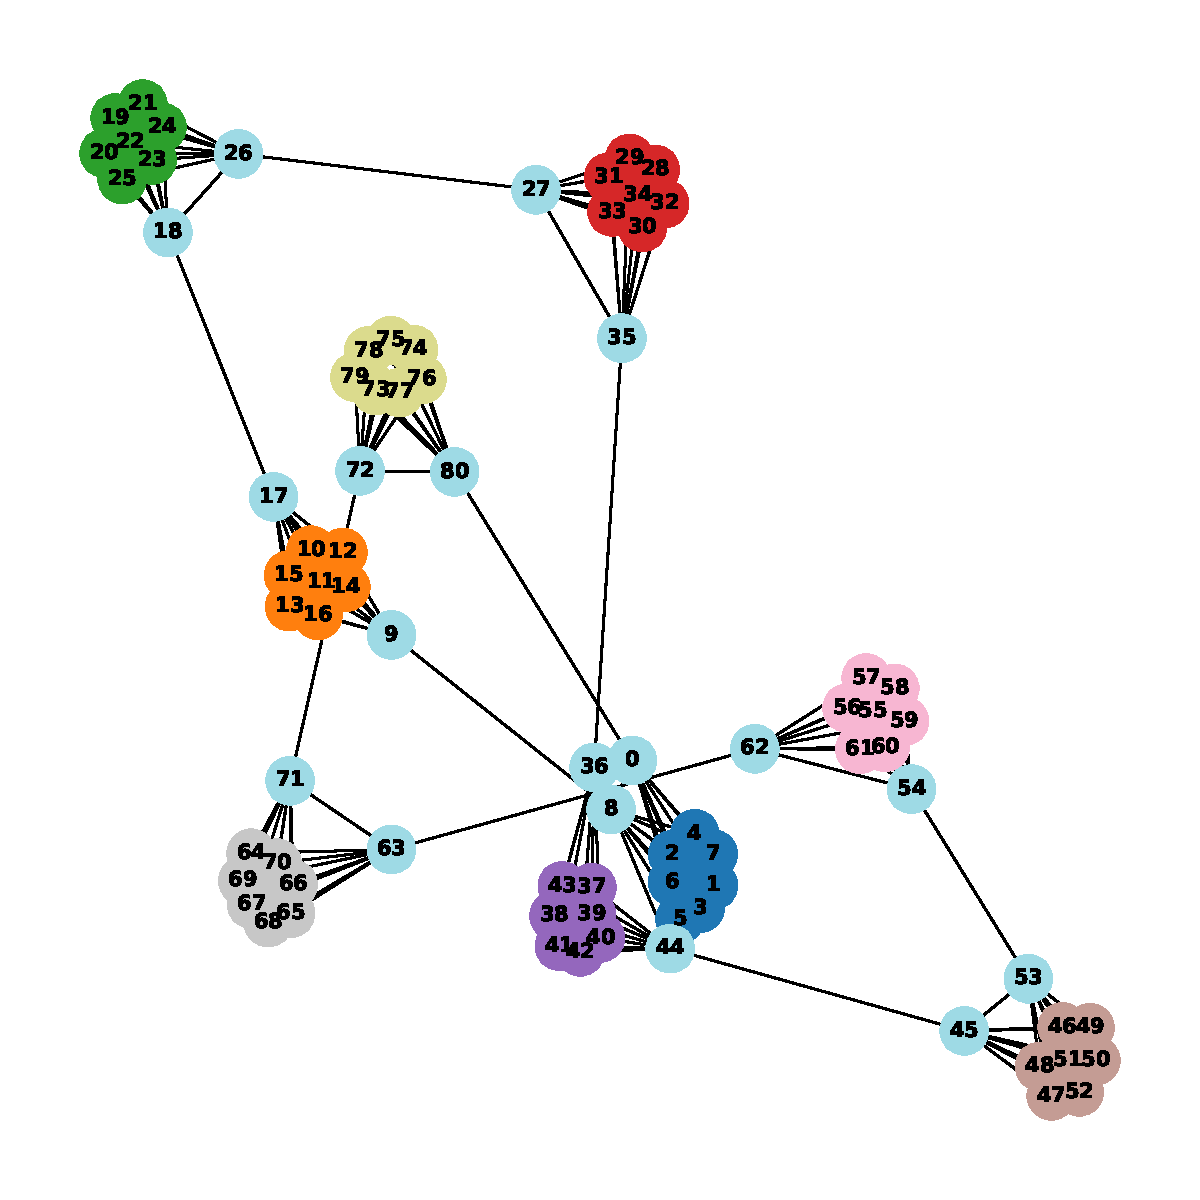
\includegraphics[width=\textwidth]{cluster_9,9newman_auto.pdf}
      \caption{9 κοινότητες από 9 κόμβους}
      \label{9b}
  \end{subfigure}
  \begin{subfigure}{0.3\textwidth}
      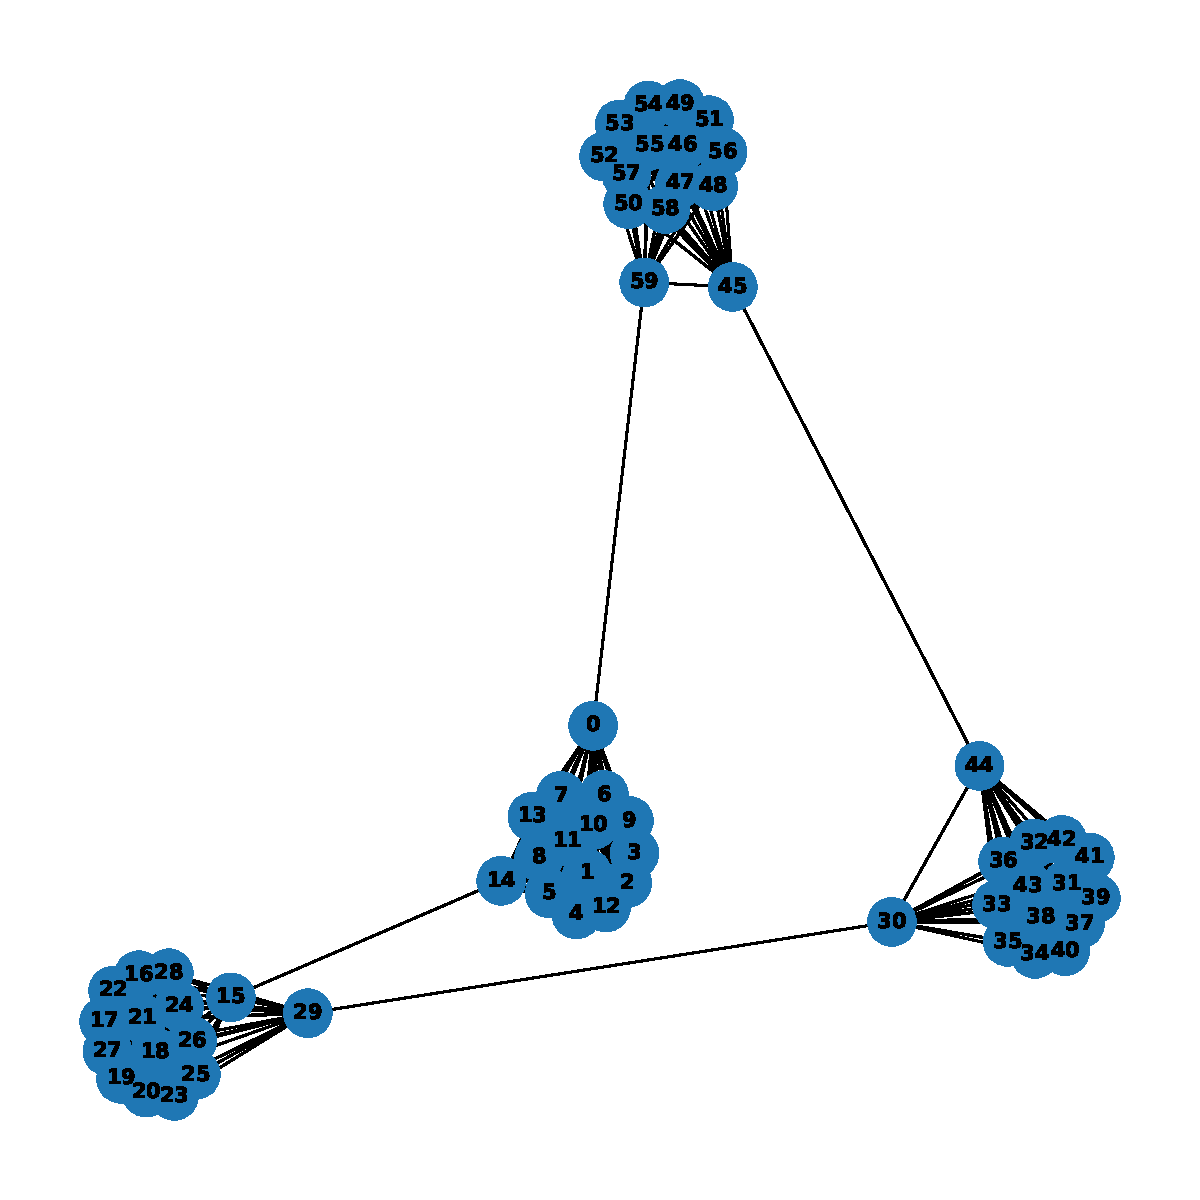
\includegraphics[width=\textwidth]{cluster_4,15newman_auto.pdf}
      \caption{4 κοινότητες από 15 κόμβους}
      \label{9c}
  \end{subfigure}
  \caption{Αλγόριθμος $Newman$ με εκτίμηση $\gamma$ από το μέγεθος των κοινοτήτων}
  \label{auto_cluster_size}
\end{figure}







Όμως το πρόβλημα έτσι δεν λύνεται: θα θέλαμε ο αλγόριθμος να μπορεί να αναγνωρίσει 
τις κοινότητες χωρίς να χρειάζεται να γνωρίζουμε ήδη το μέγεθός τους. 

% ισως συσχετηση με μεγεθος και πληθος κοινοτητων 

Μια δεύτερη παρατήρηση ήταν ότι, ενώ η βέλτιστη τιμή $\gamma$ μπορεί να αλλάξει για γράφο 
με ίδιο πλήθος κόμβων (παράδειγμα στο σχήμα \ref{ss_dcs}), φαίνεται να μένει σταθερή αν σταθεροποιήσουμε και το πόσες 
κοινότητες θα έχει. Έτσι υποθέτω ότι ίσως υπάρχει συσχέτηση με το πλήθος \emph{ακμών} του γράφου,
το οποίο εξ' άλλου γνωρίζουμε εκ των προτέρων. 

\begin{figure}
  \centering
  \begin{subfigure}{0.48\textwidth}
    \centering
    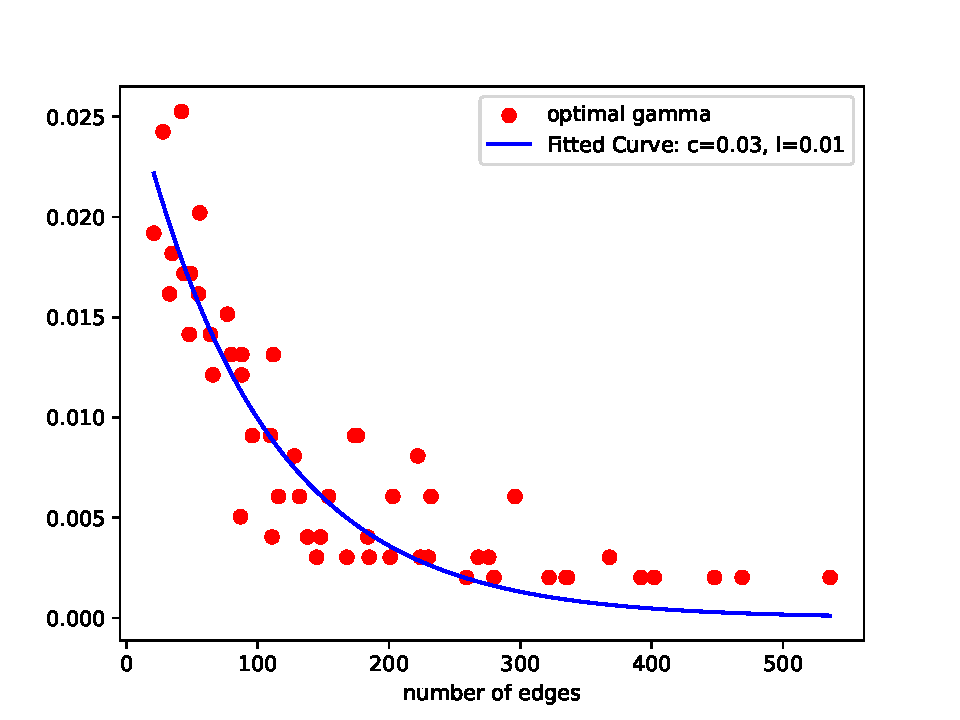
\includegraphics[width=\linewidth]{EDGES_GAMMA_FIT.pdf}
    \caption{}
    \label{EDGESFIT}
  \end{subfigure}
  \begin{subfigure}{0.48\textwidth}
    \centering
    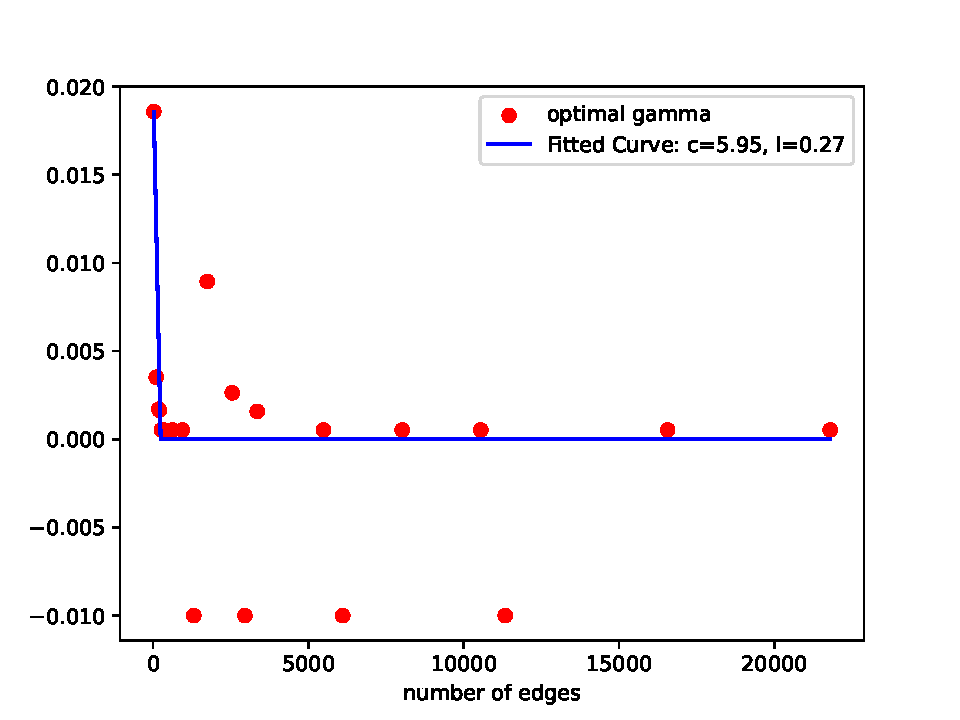
\includegraphics[width=\linewidth]{EDGES_GAMMA_FIT_noise.pdf}
    \caption{}
    \label{EDGESFIT_noise}
  \end{subfigure}
  \caption{}
\end{figure}

Οπότε για διάφορους γράφους απεικόνησα το βέλτιστο $\gamma$ ως προς το πλήθος ακμών και 
φάνηκε πάλι να υπάρχει συσχέτηση εκθετικής μείωσης. 

Στο σχήμα \ref{EDGESFIT} φαίνονται αυτά τα δεδομένα όπως και η εκτίμηση τους με την 
ίδια τεχνική όπως προηγουμένως. 

Στο σχήμα \ref{EDGESFIT_noise}, για να αντιπροσωπεύει καλύτερα ένα πραγματικό δίκτυο,
τοποθετείται \say{θόρυβος} στο γράφο, με τη μορφή ακμών που διαγράφονται από το 
εσωτερικό των κοινοτήτων και προστίθονται στο εξωτερικό τους. Έτσι μοιάζουν περισσότερο
με τους γράφους του σχήματος \ref{fig:it6} παρά αυτούς του σχήματος \ref{9b}. 
Δοκιμάστηκαν, εν τέλη, γράφοι με μεγέθη από 12 κόμβους μέχρι 1500, κοινότητες
από 3 μέχρι 50 σε πλήθος και από 4 μέχρι 30 σε μέγεθος. Σε κάθε γράφο 
οι ακμές που τοποθετούνταν τυχαία από το εσωτερικό των κοινοτήτων στο εξωτερικό τους 
ήταν $|E|/3$ σε πλήθος. Βλέπουμε (όπως ήταν και αναμενόμενο) μεγαλύτερη διασπορά 
στους τυχαίους γράφους. 



Έτσι δημιουργήθηκε μία συνάρτηση $newman\_greedy\_distance\_auto(G)$ η οποία πλέον
δέχεται ως όρισμα \emph{μόνο} τον γράφο $G$. Υπολογίζει την αναμενώμενη τιμή του $\gamma$
σύμφωνα με την εξίσωση $ce^{-\lambda |E|}$, όπου $|E|$ το πλήθος ακμών του $G$, 
$c=0.022201354581903955$, $\lambda = 0.005629355830701895$, και εκτελεί τον αλγόριθμο $Newman$ για αυτό το $\gamma$. 

Λόγω της διασποράς στο σχήματα δεν περιμένουμε να έχει πάντα το καλύτερο
αποτέλεσμα.

Αποτελέσματα της μεθόδου αυτής βρίσκονται στο σχήμα \ref{edgeresults} για διάφορα παραδείγματα. 










\begin{figure}
  \begin{subfigure}{0.5\textwidth}
    \centering
    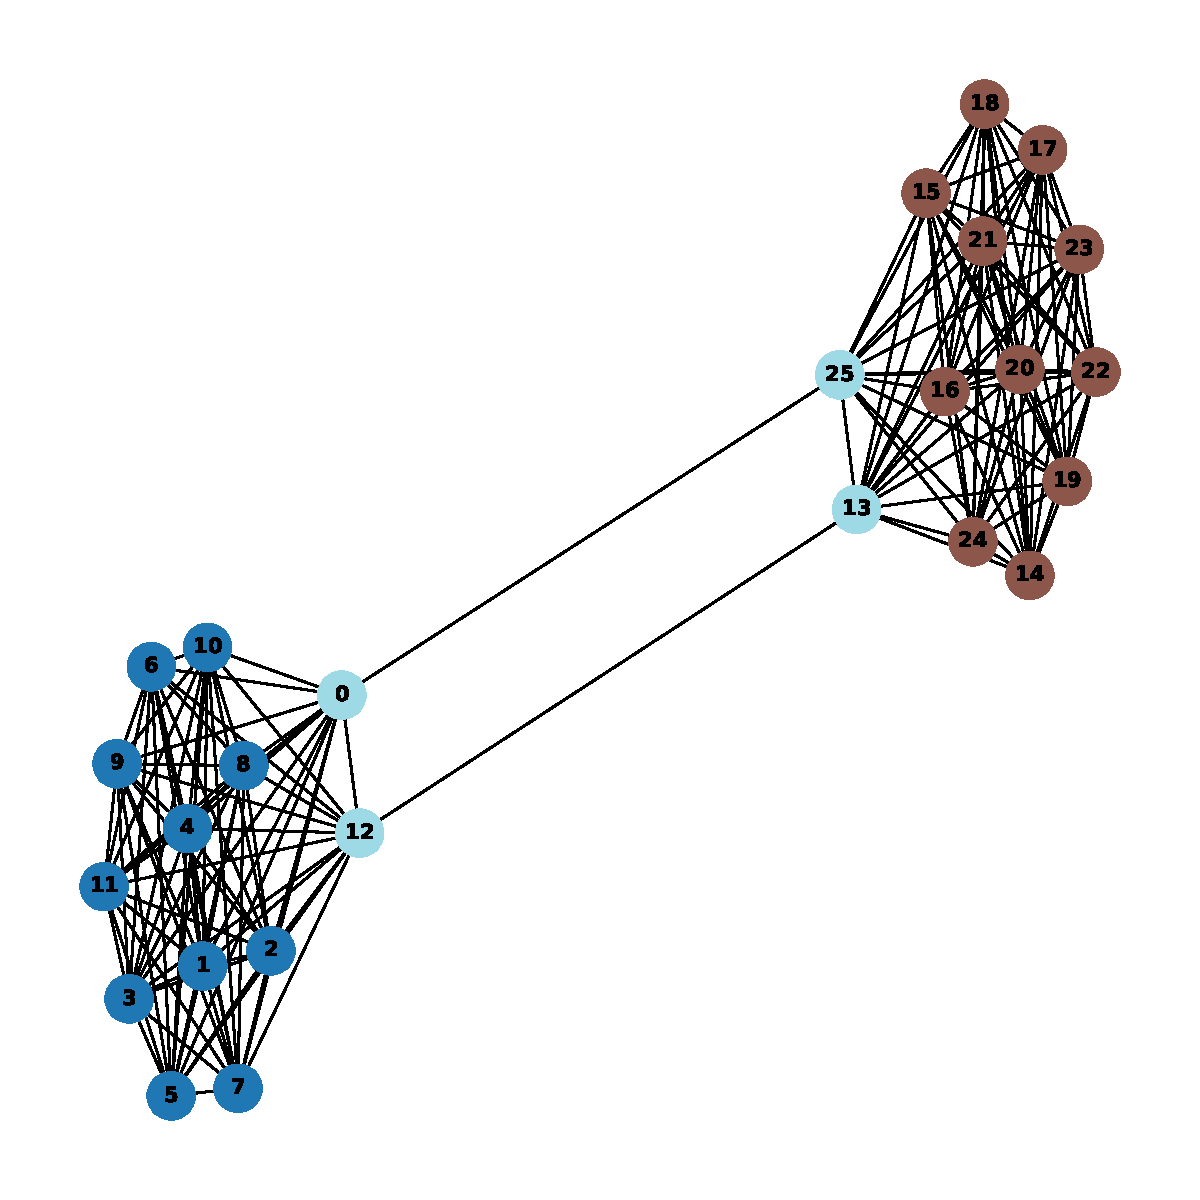
\includegraphics[width=0.8\linewidth]{AUTO2,13.pdf}
    \caption{2 κοινότητες 13 κόμβων}
    \label{}
  \end{subfigure}
  \begin{subfigure}{0.5\textwidth}
    \centering
    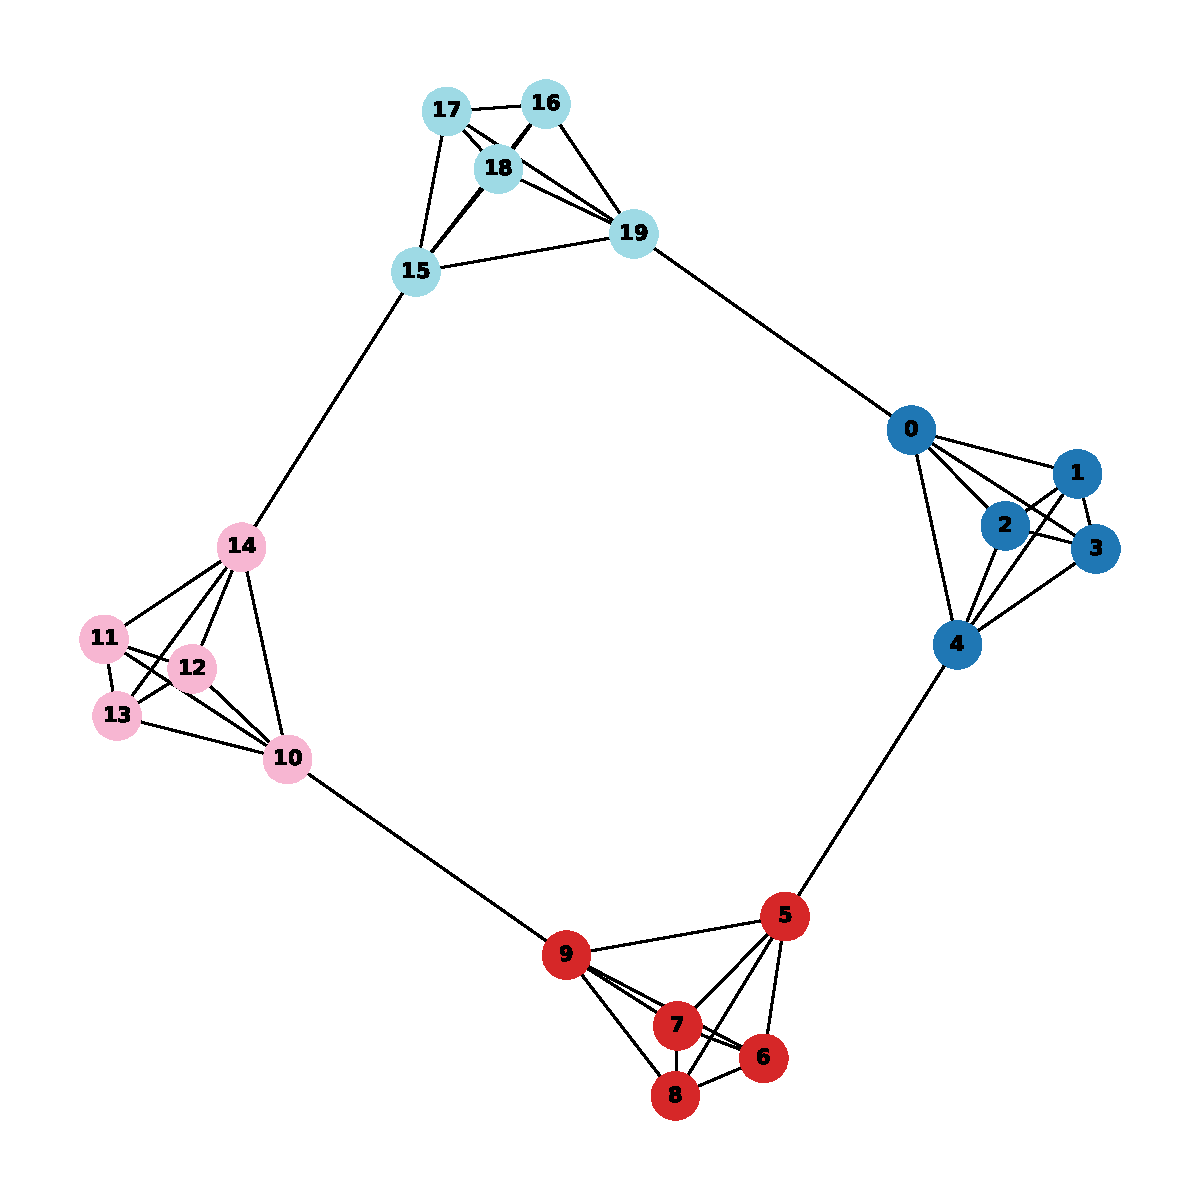
\includegraphics[width=0.8\linewidth]{AUTO4,5.pdf}
    \caption{4 κοινότητες 5 κόμβων}
    \label{}
  \end{subfigure}

  \vfill

  \begin{subfigure}{0.5\textwidth}
    \centering
    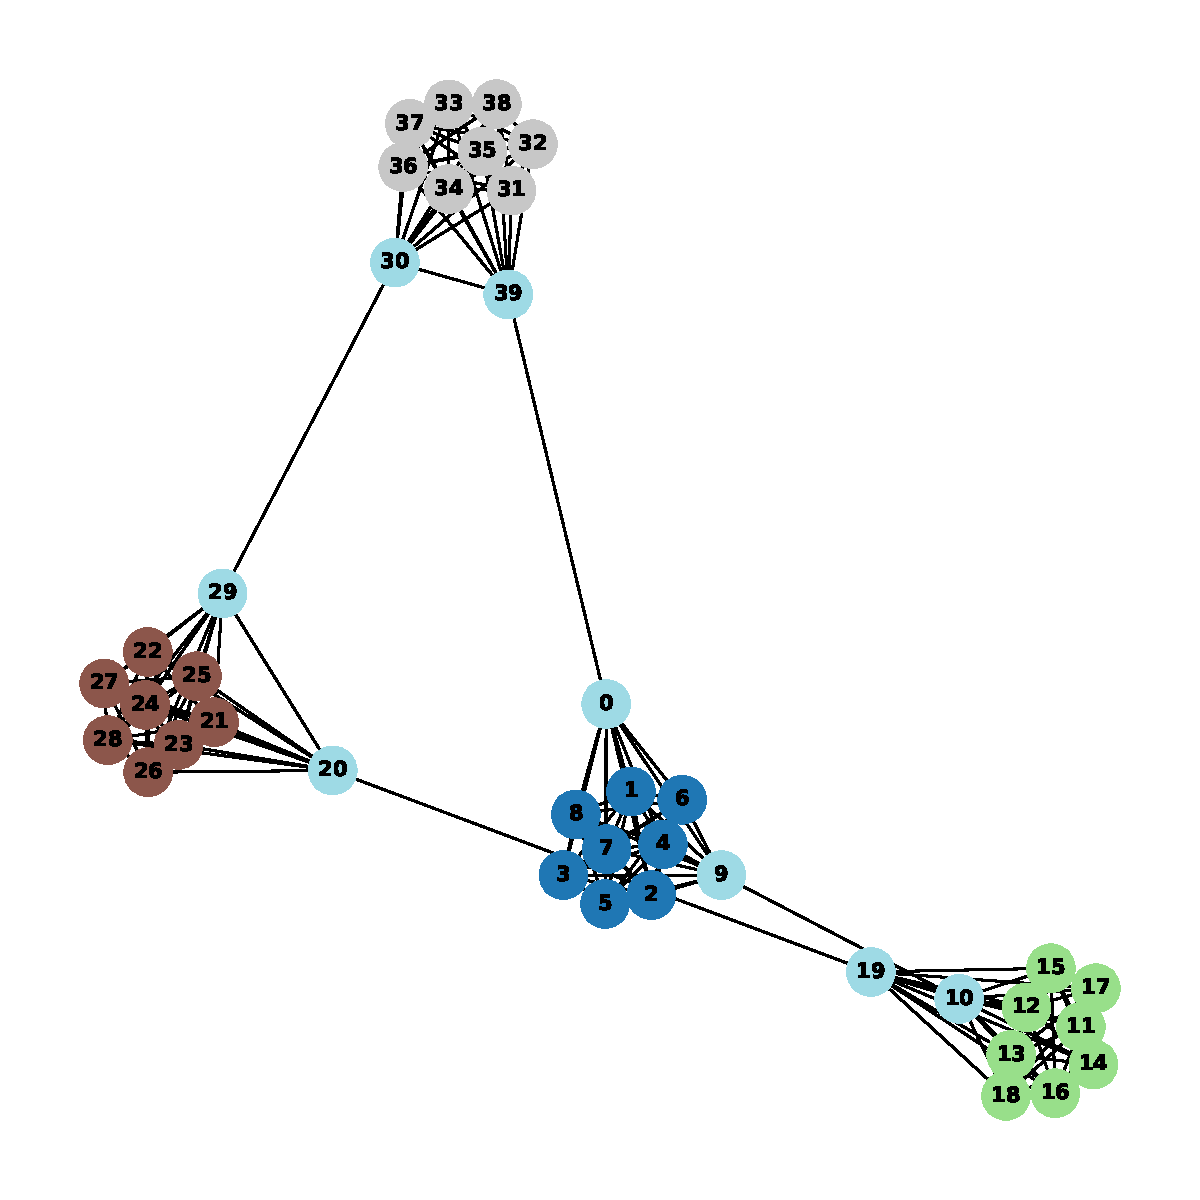
\includegraphics[width=0.8\linewidth]{AUTO4,10.pdf}
    \caption{4 κοινότητες 10 κόμβων}
    \label{}
  \end{subfigure}
  \begin{subfigure}{0.5\textwidth}
    \centering
    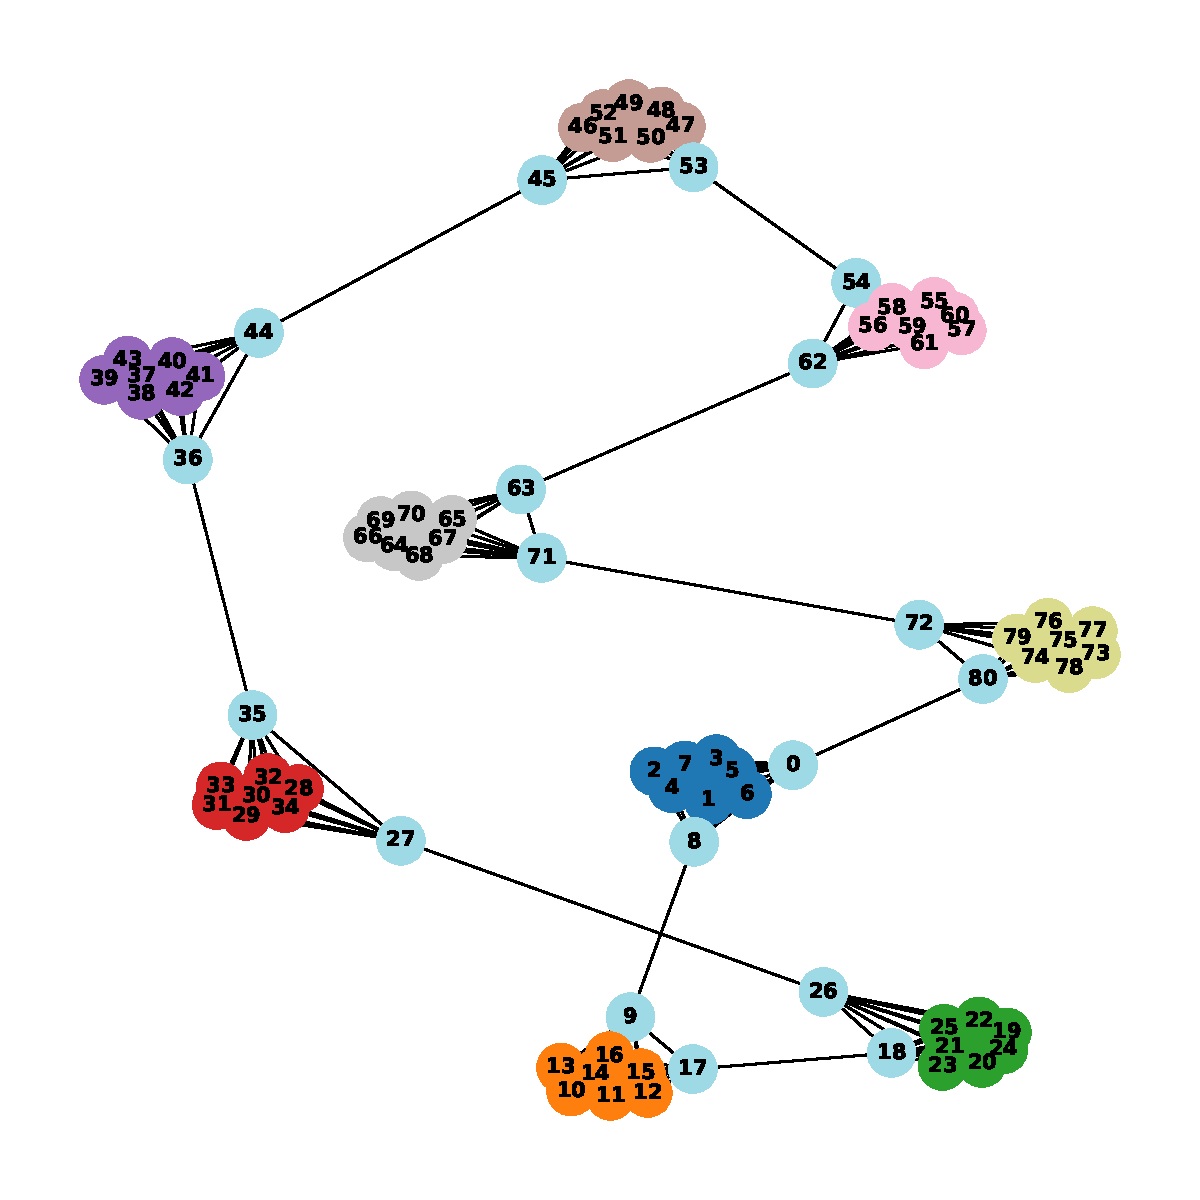
\includegraphics[width=0.8\linewidth]{AUTO9,9.pdf}
    \caption{9 κοινότητες 9 κόμβων}
    \label{}
  \end{subfigure}


  \caption{Αποτελέσματα της μεθόδου εκτίμησης του $\gamma$
  από το πλήθος ακμών, για διάφορους γράφους.}
  \label{edgeresults}
\end{figure}














\subsection{Ανικανότητες των τεχνικών αξιολόγησης}

Για την αξιολόγηση του $Q_d$ ως μετρηκή για αναγνώρηση κοινοτήτων χρησιμοποιήσαμε 
μόνο γράφους των οποίων οι κοινότητες έχουν ίδιο μέγεθος, και 
είναι στενά συνδεδεμένες και πολύ αποσυνδεδεμένες μεταξύ τους. 
Τέτοια δίκτυα δύσκολα παρατηρούνται στον πραγματικό κόσμο. 

Υπάρχουν πιο ρεαλιστικές τεχνικές αξιολόγησης \cite{benchmark_realistic} οι οποίες δεν 
ήταν στα πλαίσια της παρούσης εργασίας. 


Η μετρηκή $Q_d$ (\textlatin{distance quiality}) δεν φαίνεται να λειτουργεί καλά για γράφους
των οποίων οι κοινότητες δεν έχουν ίδια μεγέθη. 
Ένα παράδειγμα φαίνεται στο σχήμα \ref{different_sizes}.  

Είναι πιθανό, τέλος, επειδή τα δεδομένα συσχέτησης του βέλτιστου $\gamma$ με το πλήθος 
ακμών παράχθηκαν με τέτοιους γράφους, η συσχέτηση αυτή να μην ανταποκρίνεται στην πραγματικότητα. 



\begin{figure}
  \centering
  \begin{subfigure}{0.3\linewidth}
      \centering
      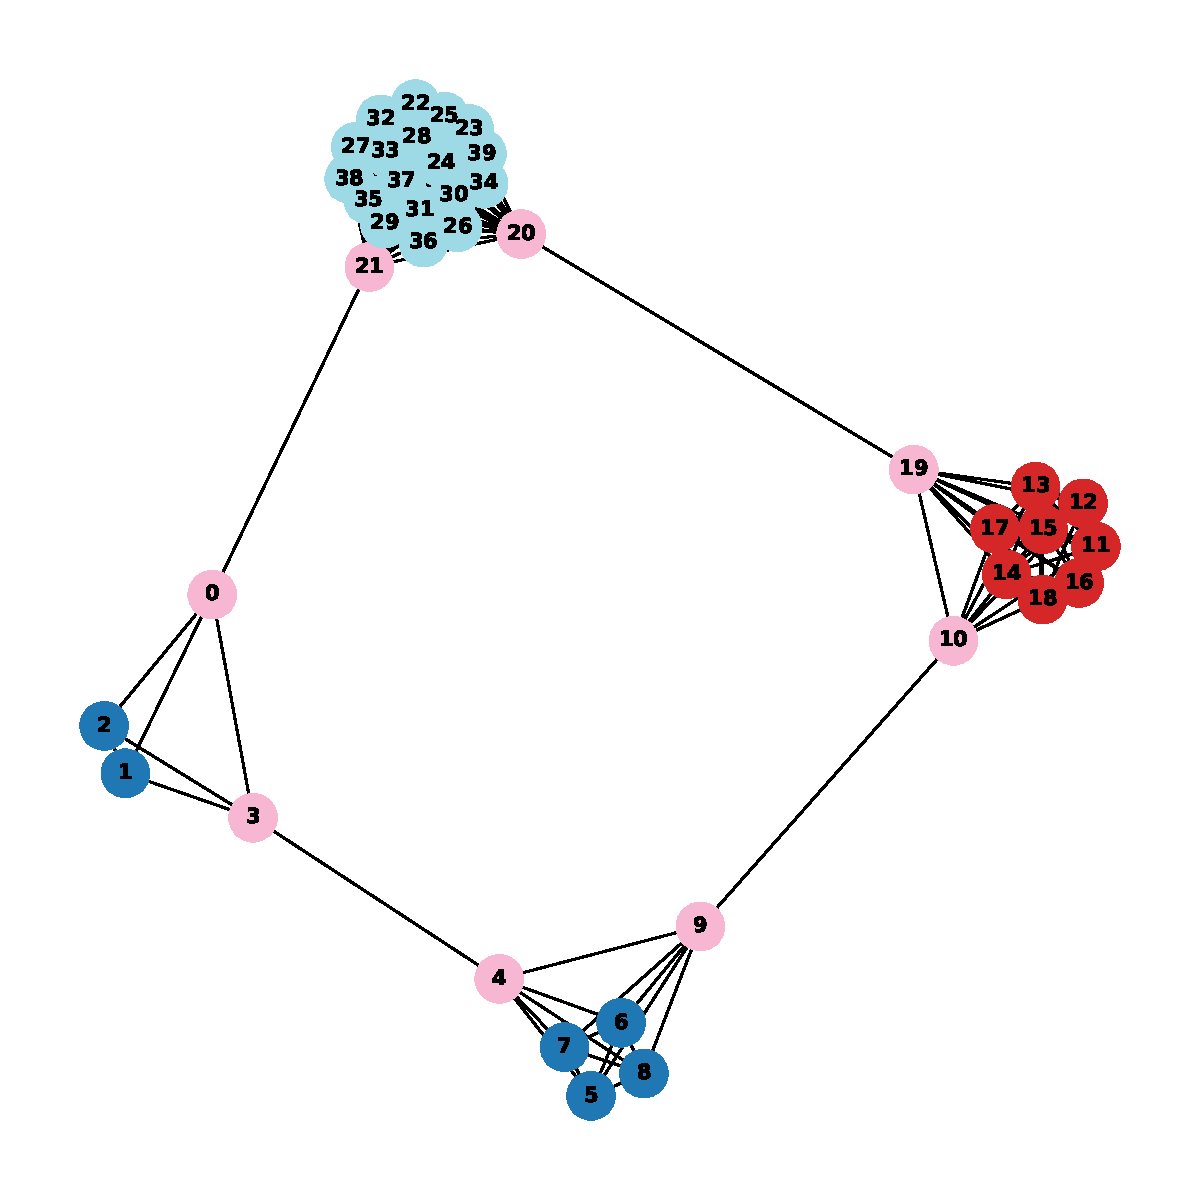
\includegraphics[width=\linewidth]{different_size_communities.pdf}
      \caption{Γράφος με κοινότητες διαφορετικών μεγεθών.}
      \label{different_sizes}
  \end{subfigure}
  \begin{subfigure}{0.66\linewidth}
    \centering
    \begin{subfigure}{0.45\linewidth}
        \centering
        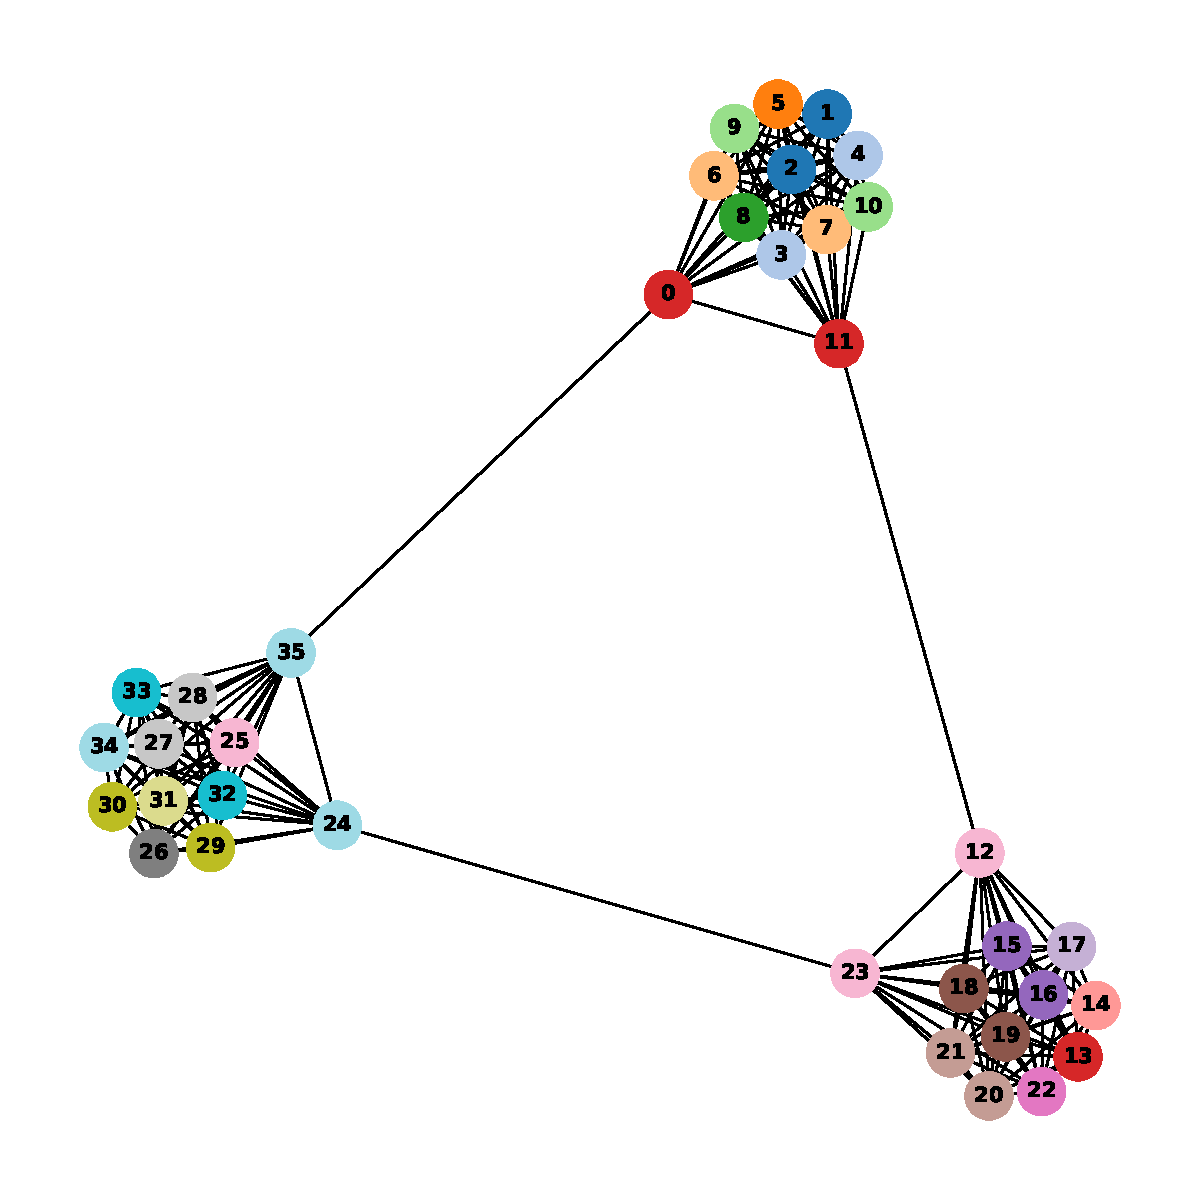
\includegraphics[width=\linewidth]{nonconnected_ssize_dcs0.011.pdf}
        \label{}
    \end{subfigure}
    \begin{subfigure}{0.45\linewidth}
        \centering
        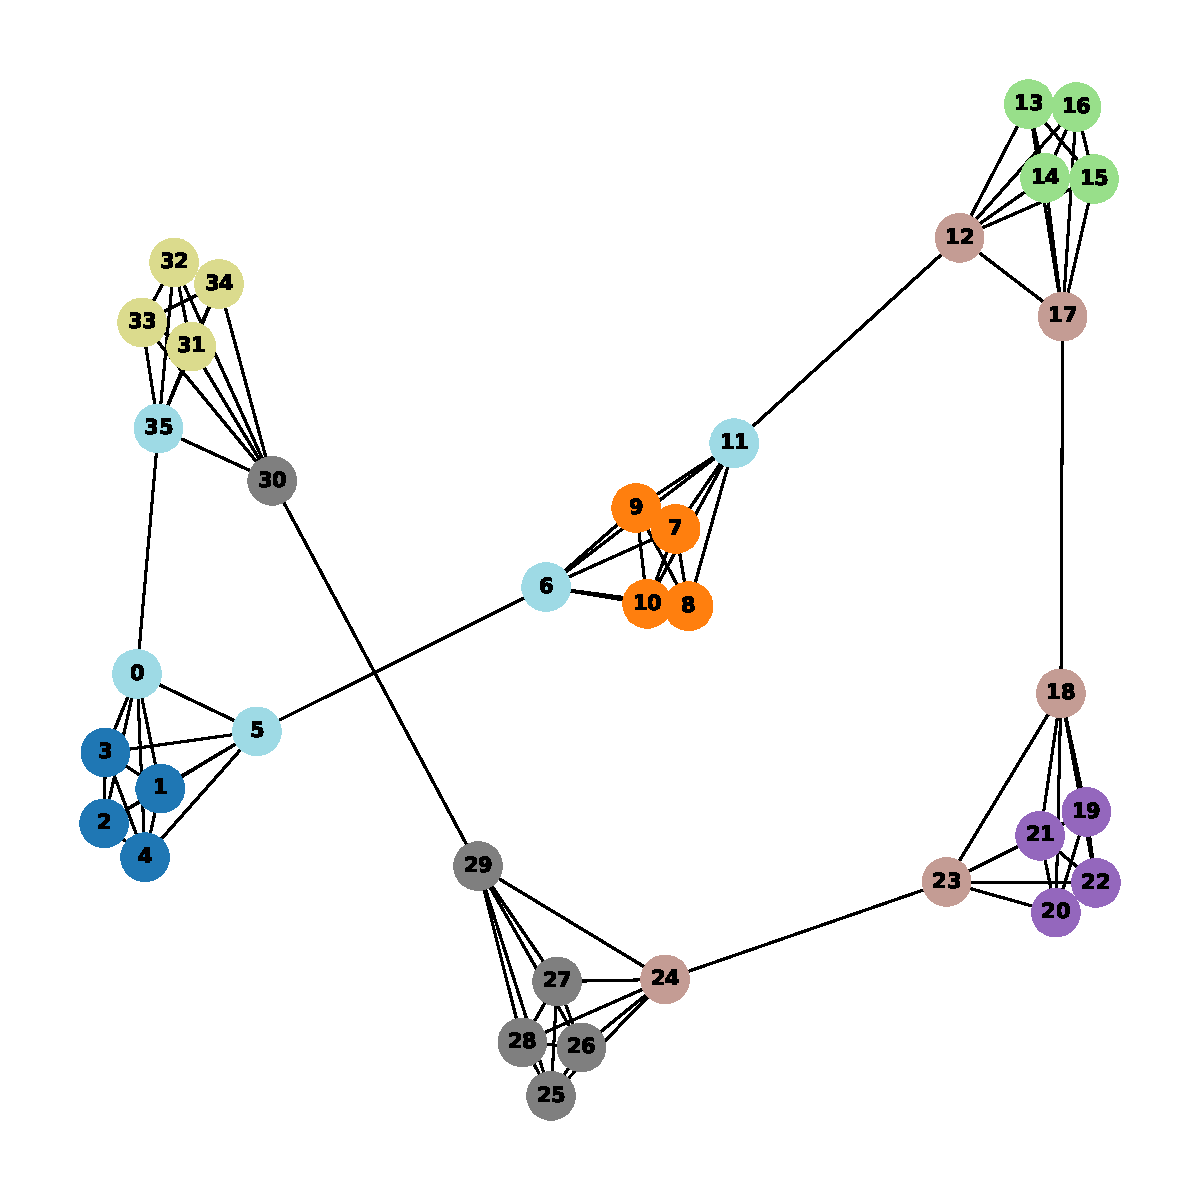
\includegraphics[width=\linewidth]{nonconnected_ssize_dcs0.012.pdf}
        \label{}
    \end{subfigure}
    \caption{Οι δύο γράφοι έχουν το ίδιο μέγεθος (πλήθος κόμβων), όμως με την ίδια τιμή 
    $\gamma = 0.01$ στον πρώτο δεν αναγνωρίζονται οι κοινότητες ενώ στον δεύτερο γίνεται 
    μια καλή προσπάθεια.}
    \label{ss_dcs}
  \end{subfigure}
  \caption{}
  \label{endplots}
\end{figure}









\section{Πραγματικός γράφος}





Θε ελέγξουμε, επιτέλους, την απόδοση της $Q_d$ σε έναν πραγματικό δίκτυο. 
Χρησιμοποιήθηκε το δίκτυο \href{https://snap.stanford.edu/data/email-Eu-core.html}{
  \textlatin{email-Eu-core network}
} απο το \href{https://snap.stanford.edu/index.html}{\textlatin{Stanford Network Analysis Project}},
το οποίο αντιπροσωπεύει επικοινωνία δύο μελών ενός Ευρωπαϊκού ινστιτούτου
έρευνας μέσω \textlatin{e-mail}. 
Αποτελείται από 1005 κόμβους και 25571 ακμές.
Μας δίνονται επίσης οι πραγματικές κοινότητες (42 τμήματα στα οποία ανήκουν).







Στο σχήμα \ref{Eu-real} αποτυπώνεται το δίκτυο και οι σημαντικότερες κοινότητες του 
χρωματίζονται.


Είναι κατευθυνόμενο, όμως επειδή όλα τα παραπάνω αναπτύχθηκαν για ακατεύθυντους γράφους,
θα το μετατρέψουμε σε ακατεύθυντο για την αναγνώρηση κοινοτήτων.


Δοκιμάστηκε ο αλγόριθμος που υπολογίζει το αναμενόμενο $\gamma$ σύμφωνα με το πλήθος 
ακμών. Τα αποτελέσματα βρίσκονται στο σχήμα \ref{Eu-expected}, όπως φαίνεται είναι πολύ κακά.
Ταξινομεί σχεδόν όλους τους γράφους στην ίδια κοινότητα.
Ίσως η μέθοδος αυτή να μην μπορεί να λειτουργήσει εξ' αιτίας τις διασποράς του βέλτιστου 
$\gamma$, αλλά ίσως και με καλύτερα δεδομένα και καλύτερη εκπαίδευση να μπορεί να βγάλει καλύτερα
αποτελέσματα.


Έπειτα δοκιμάστηκε ο αλγόριθμος $Newman$ με $\gamma = 0.000007$. Τα αποτελέσματα βρίσκονται 
στο σχήμα \ref{Eu-gamma}. Εδώ έχει αναγνωρίσει κάποιες κοινότητες, οι οποίες θυμίζουν σε έναν 
μικρό βαθμό τις πραγματικές, όμως τα αποτελέσματα δεν είναι σε καμία περίπτωση 
χρήσιμα. Οι πραγματικές με τις υπολογισμένες κοινότητες έχουν $Jaccard \ similarity \approx 0.2$.

Στην υλοποίηση μου, ο αλγόριθμος τερματίζει στα 10 δευτερόλεπτα για τον πραγματικό γράφο.

Για σύγκριση δοκιμάστηκε στον ίδιο γράφο η \textlatin{modularity}. Τα αποτελέσματα βρίσκονται στο σχήμα 
\ref{Eu-modularity}.
Αξιοσημείωτο ότι η ομοιότητα \textlatin{Jaccard} πραγματικών κοινοτήτων με τη \textlatin{modularity} είναι μικρότερη 
από ότι με την \textlatin{distance} ($\approx 0.1$). 



\begin{figure}
  \centering
  \includegraphics[width=0.6\textwidth]{../gephi/email-Eu-core.pdf}
  \caption{Πραγματικό δίκτυο, χρωματισμένες είναι οι (βασικές) πραγματικές κοινότητές του.
  Το μέγεθος των κόμβων καθορίζεται από τον βαθμό τους.}
  \label{Eu-real}
\end{figure}


\begin{figure}
  \centering
  \includegraphics[width=0.6\textwidth]{../gephi/email-Eu-core-calculated-expectedgamma.pdf}
  \caption{Πραγματικό δίκτυο, χρωματισμένες είναι οι κοινότητες που υπολογίστηκαν με το 
  αναμενόμενο $\gamma$ σε σχέση με το πλήθος των ακμών.}
  \label{Eu-expected}
\end{figure}

\begin{figure}
  \centering
  \includegraphics[width=0.6\textwidth]{../gephi/email-Eu-core-calculated-gamma=0.000007.pdf}
  \caption{Πραγματικό δίκτυο, χρωματισμένες είναι οι κοινότητες που υπολογίστηκαν με $\gamma = 0.000007$}
  \label{Eu-gamma}
\end{figure}

\begin{figure}
  \centering
  \includegraphics[width=0.6\textwidth]{../gephi/email-Eu-core-modularity.pdf}
  \caption{Πραγματικό δίκτυο, χρωματισμένες είναι οι κοινότητες που υπολογίστηκαν με \textlatin{modularity}.}
  \label{Eu-modularity}
\end{figure}


\pagebreak

\section{Συμπεράσματα}


Η συγκεκριμένη παραλλαγή της \textlatin{distance quality function}, ενώ καταφέρνει να 
παράγει κάποια αποτελέσματα, δεν είναι ικανοποιητικά για χρήση σε πραγματικά δίκτυα. 


Μπορεί με παραπάνω προσπάθεια να υποστεί βελτίωση, όμως θεωρώ 
ότι προτιμότερο θα ήταν θα ελεγθεί κάποια διαφορετική παραλλαγή της. Παραδείγματως χάρη 
αυτή που λειτουργεί με τεχνική \textlatin{random walk} φαίνεται να έχει καλά αποτελέσματα 
(όπως φαίνεται στο γράφημα με σύγκριση των μεθόδων στις σημειώσεις του μαθήματος).




\section{Σημειώσεις περί του κώδικα}

Συμπεριλαμβάνονται 12 αρχεία κώδικα, τα οποία διαχωρίζω σε 3 κατηγορίες 

\begin{enumerate}
  \item Σημαντικά αρχεία: αυτά που περιέχουν τον πηγαίο κώδικα για τις μεθόδους που περιγράφτηκαν.
  \item Αναγκαία αρχεία: αυτά που περιέχουν κάποιες συναρτήσεις που χρησιμοποιούν τα υπόλοιπα.
  \item Αρχεία τεστ: αρχεία στα οποία δοκιμάστηκαν παραδείγματα, \textlatin{benchmarks}, κλπ.
\end{enumerate}

Αναλυτική περιγραφή για αυτά και το $gephi$ υπάρχει στο $README.txt$ που θα βρείτε στον φάκελο.



\selectlanguage{english}
\renewcommand{\refname}{\selectlanguage{greek} Αναφορές}  
\bibliographystyle{plain}
\bibliography{sources.bib}



\end{document}
